\chapter{DREAD/NOUGHT} 
\label{sec:baydoor}
\lstset{style=6502Style}

The levels in Uridium are beautiful things. But we never get to take them in all at
once. Here are a selection, shrunk down to fit a page.
\begin{figure}[H]
    \centering
    \begin{adjustbox}{width=13cm,center}
      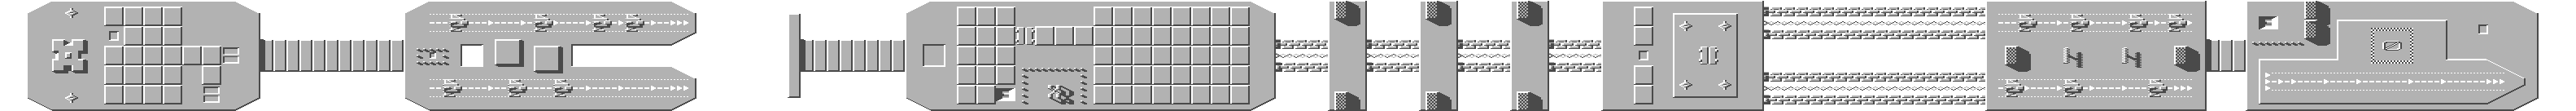
\includegraphics[width=15cm]{src/surfaces_raw/1.png}%
    \end{adjustbox}
\end{figure}
\vspace{-0.6cm}
\begin{figure}[H]
    \centering
    \begin{adjustbox}{width=13cm,center}
      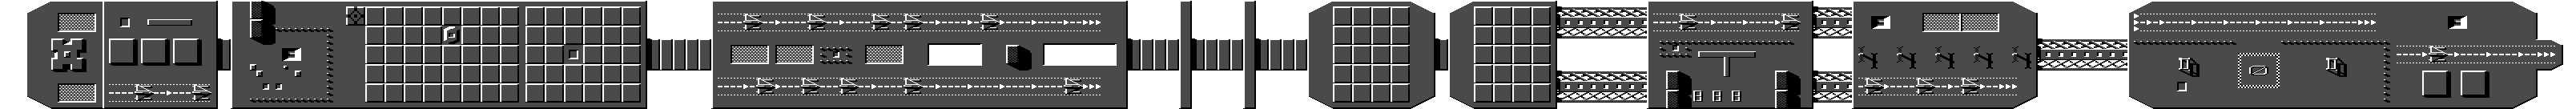
\includegraphics[width=15cm]{src/surfaces_raw/2.png}%
    \end{adjustbox}
\end{figure}
\vspace{-0.6cm}
\begin{figure}[H]
    \centering
    \begin{adjustbox}{width=13cm,center}
      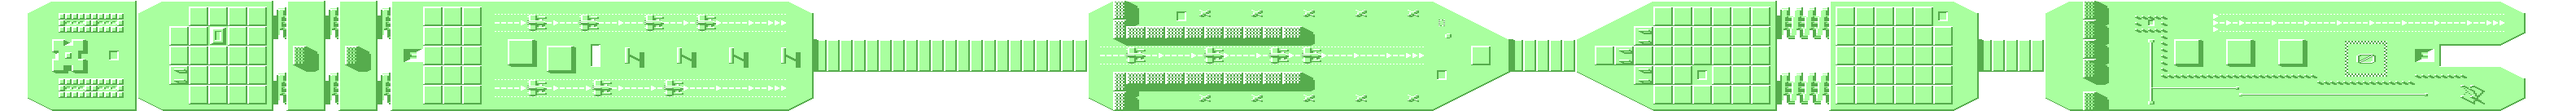
\includegraphics[width=15cm]{src/surfaces_raw/5.png}%
    \end{adjustbox}
\end{figure}
\vspace{-0.6cm}
\begin{figure}[H]
    \centering
    \begin{adjustbox}{width=13cm,center}
      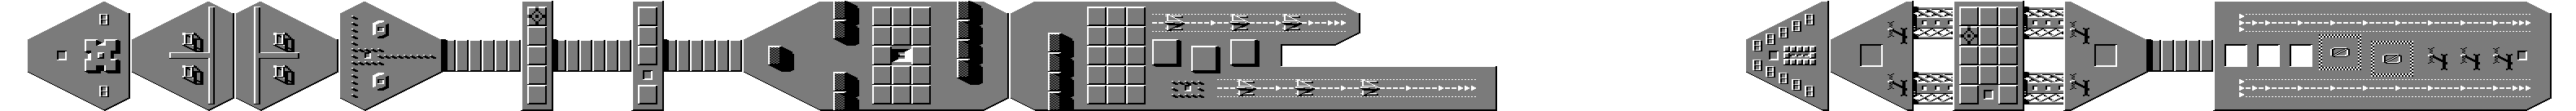
\includegraphics[width=15cm]{src/surfaces_raw/8.png}%
    \end{adjustbox}
\end{figure}
\vspace{-0.6cm}
\begin{figure}[H]
    \centering
    \begin{adjustbox}{width=13cm,center}
      
\includegraphics[width=15cm]{src/surfaces_raw/9.png}%
    \end{adjustbox}
\end{figure}
\vspace{-0.6cm}
\begin{figure}[H]
    \centering
    \begin{adjustbox}{width=13cm,center}
      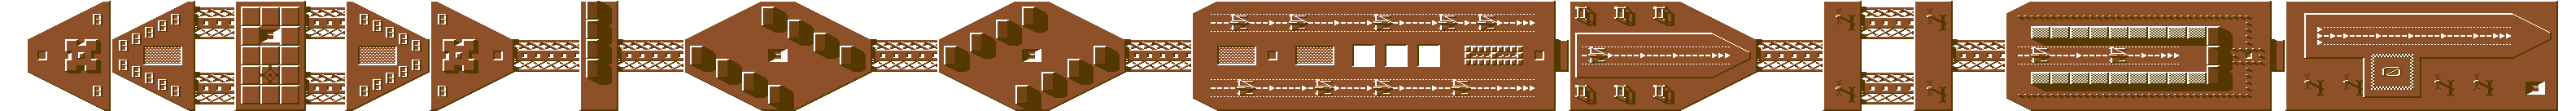
\includegraphics[width=15cm]{src/surfaces_raw/11.png}%
    \end{adjustbox}
\end{figure}
\vspace{-0.6cm}
\begin{figure}[H]
    \centering
    \begin{adjustbox}{width=13cm,center}
      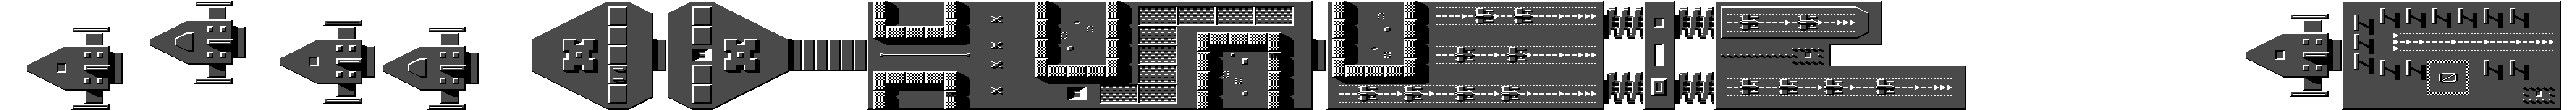
\includegraphics[width=15cm]{src/surfaces_raw/13.png}%
    \end{adjustbox}
\end{figure}

Let's zoom in a bit and see what they look like closer up.

%\raisebox{-0.3\totalheight}{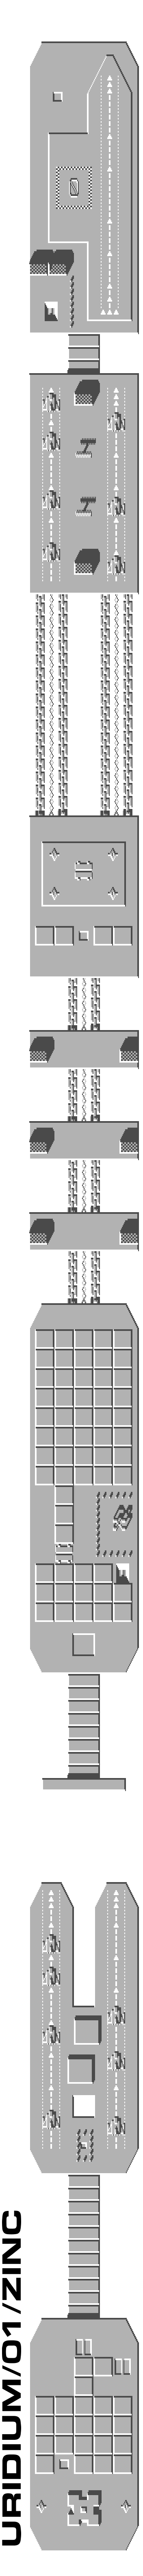
\includegraphics[height=18.5cm]{src/surface_diagrams/1.png}}
%\hspace{0.1cm}
%\raisebox{-0.3\totalheight}{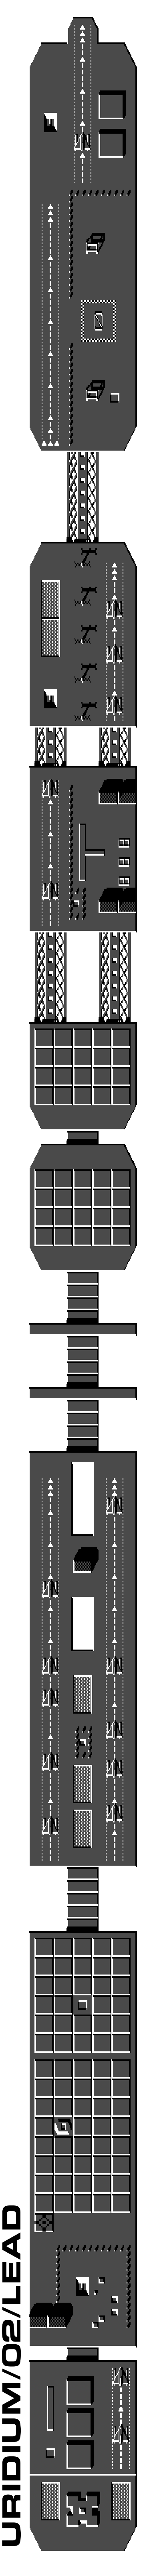
\includegraphics[height=18.5cm]{src/surface_diagrams/2.png}}
%\hspace{0.1cm}
%\raisebox{-0.3\totalheight}{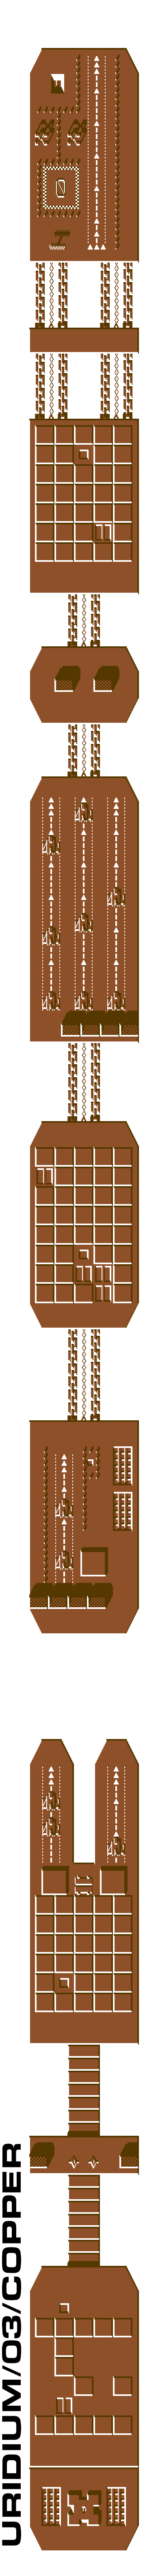
\includegraphics[height=18.5cm]{src/surface_diagrams/3.png}}
%\hspace{0.1cm}
%\raisebox{-0.3\totalheight}{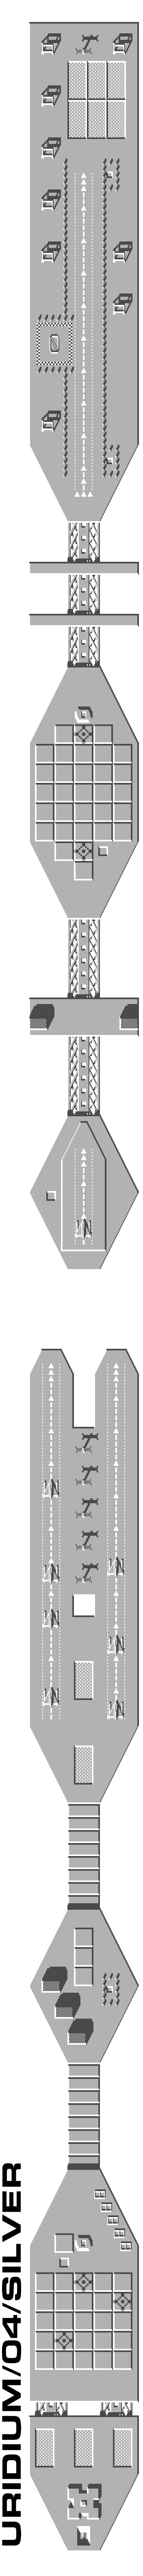
\includegraphics[height=18.5cm]{src/surface_diagrams/4.png}}
%\hspace{0.1cm}
%\raisebox{-0.3\totalheight}{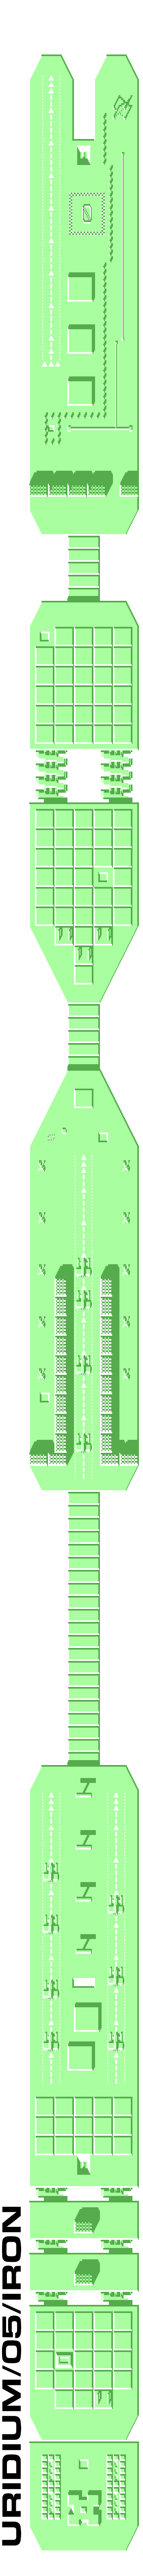
\includegraphics[height=18.5cm]{src/surface_diagrams/5.png}}
%\hspace{0.1cm}
%\raisebox{-0.3\totalheight}{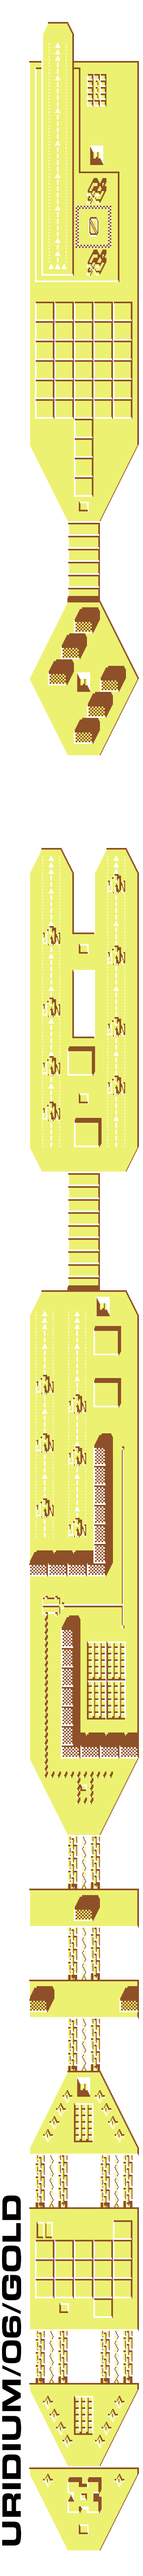
\includegraphics[height=18.5cm]{src/surface_diagrams/6.png}}
%\hspace{0.1cm}
%\raisebox{-0.3\totalheight}{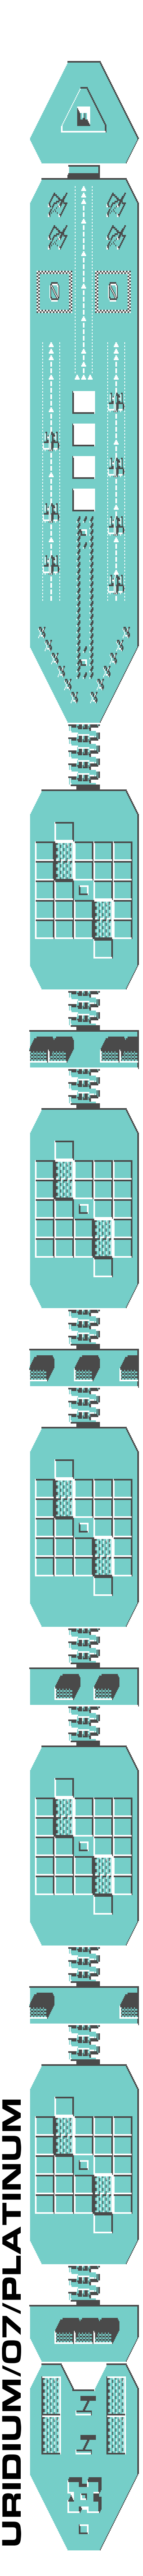
\includegraphics[height=18.5cm]{src/surface_diagrams/7.png}}
%\hspace{0.1cm}
%\raisebox{-0.3\totalheight}{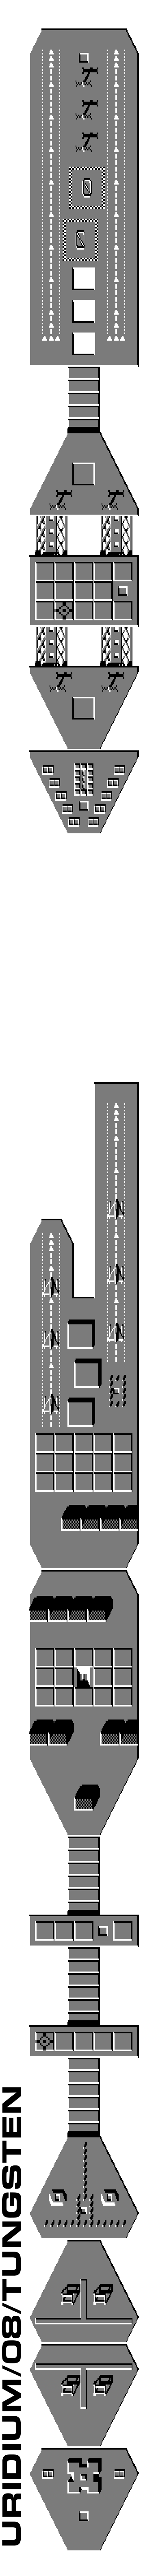
\includegraphics[height=18.5cm]{src/surface_diagrams/8.png}}
%\hspace{0.1cm}
%\raisebox{-0.3\totalheight}{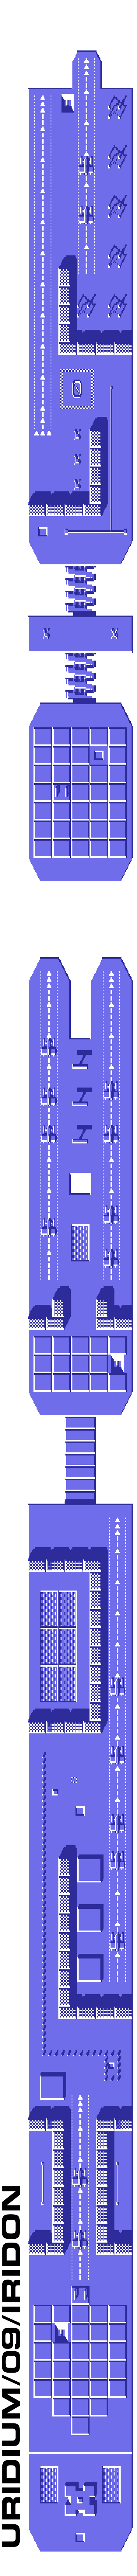
\includegraphics[height=18.5cm]{src/surface_diagrams/9.png}}
%\hspace{0.1cm}
%\raisebox{-0.3\totalheight}{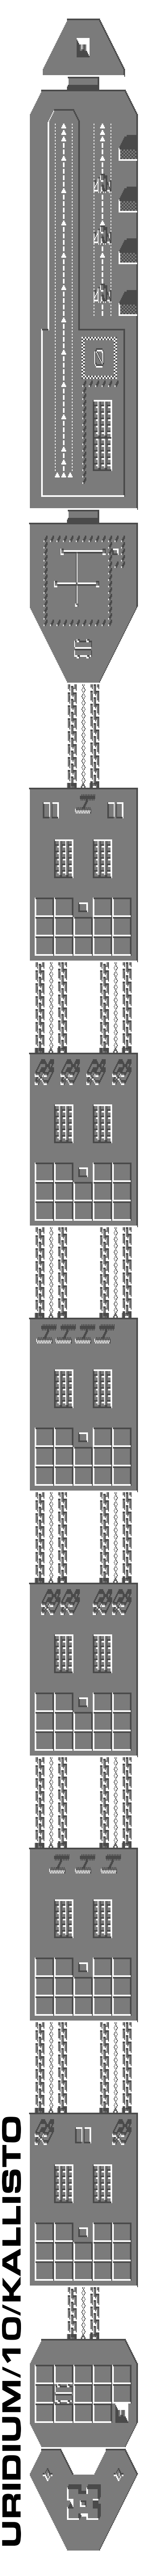
\includegraphics[height=18.5cm]{src/surface_diagrams/10.png}}
%\hspace{0.1cm}
%\raisebox{-0.3\totalheight}{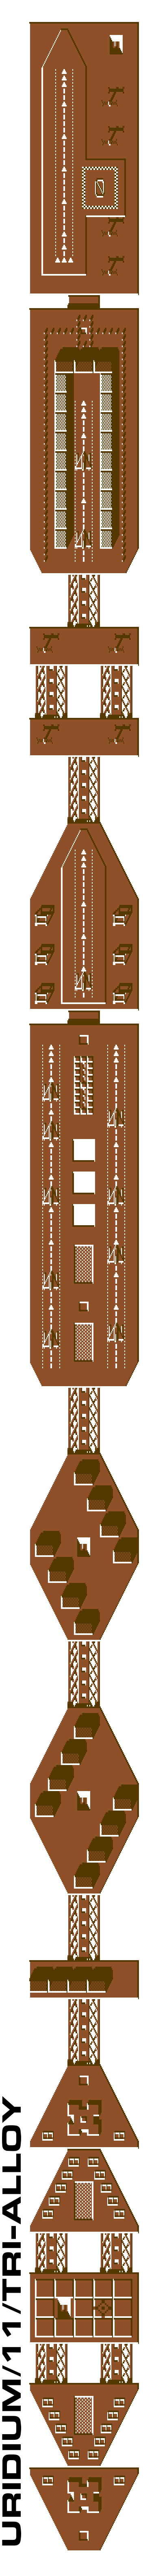
\includegraphics[height=18.5cm]{src/surface_diagrams/11.png}}
%\hspace{0.1cm}
%\raisebox{-0.3\totalheight}{
\includegraphics[height=18.5cm]{src/surface_diagrams/12.png}}
%\hspace{0.1cm}
%\raisebox{-0.3\totalheight}{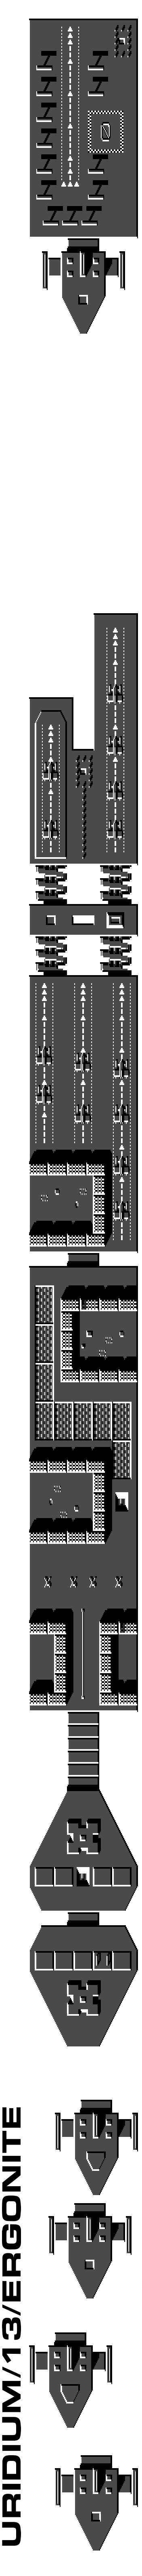
\includegraphics[height=18.5cm]{src/surface_diagrams/13.png}}
%\hspace{0.1cm}
%\raisebox{-0.3\totalheight}{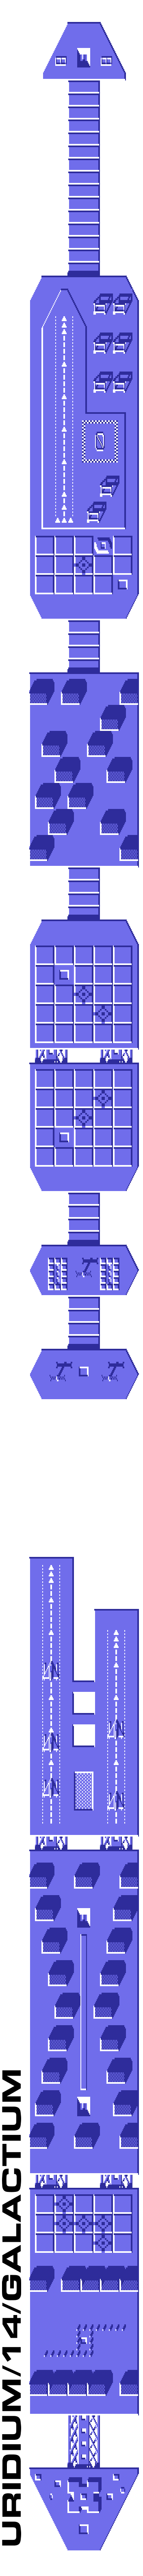
\includegraphics[height=18.5cm]{src/surface_diagrams/14.png}}
%\hspace{0.1cm}
%\raisebox{-0.3\totalheight}{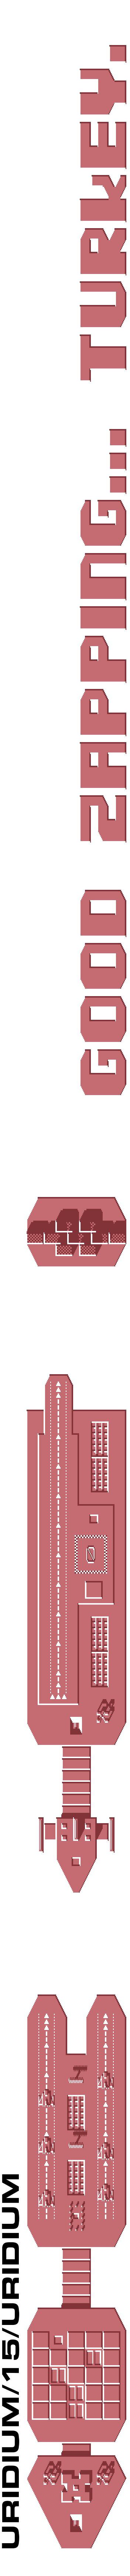
\includegraphics[height=18.5cm]{src/surface_diagrams/15.png}}
%\clearpage
%

\clearpage
\begin{figure}[H]
    \begin{adjustbox}{height=1.8cm,left}
      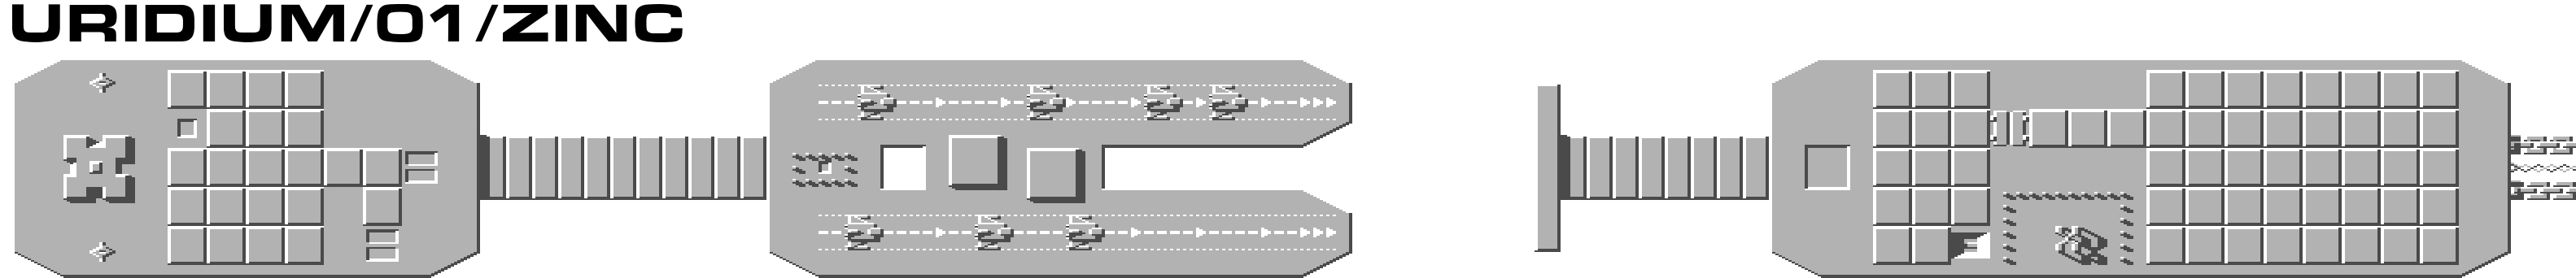
\includegraphics{src/surface_diagrams/1_horizontal_1.png}%
    \end{adjustbox}
\end{figure}
\vspace{-0.1cm}
\begin{figure}[H]
    \begin{adjustbox}{height=1.8cm,left}
      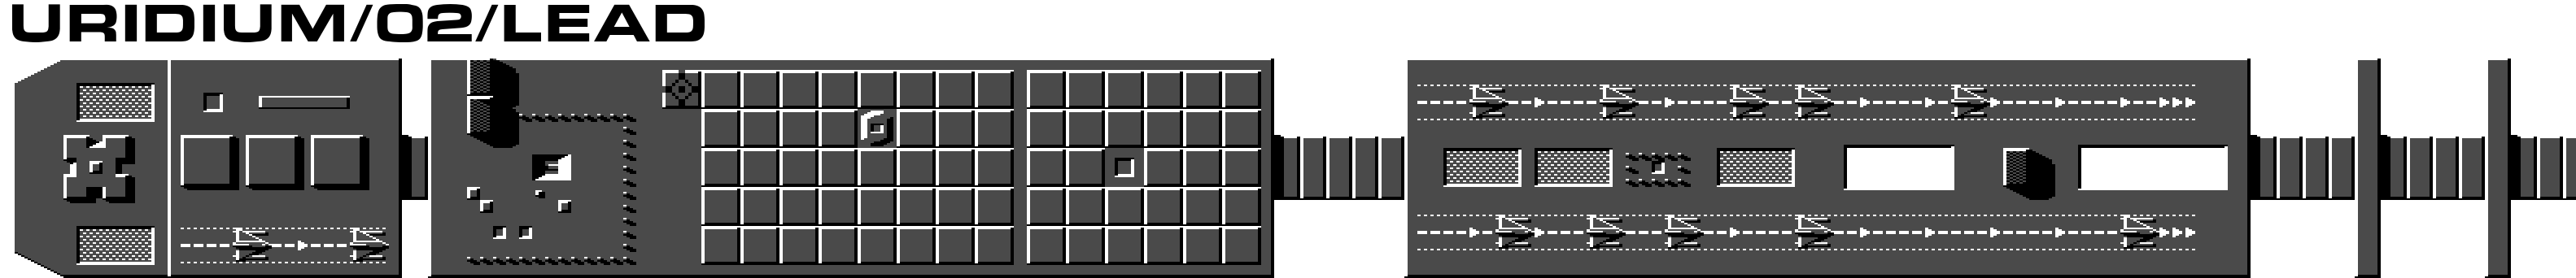
\includegraphics{src/surface_diagrams/2_horizontal_1.png}%
    \end{adjustbox}
\end{figure}
\vspace{-0.1cm}
\begin{figure}[H]
    \begin{adjustbox}{height=1.79cm,left}
      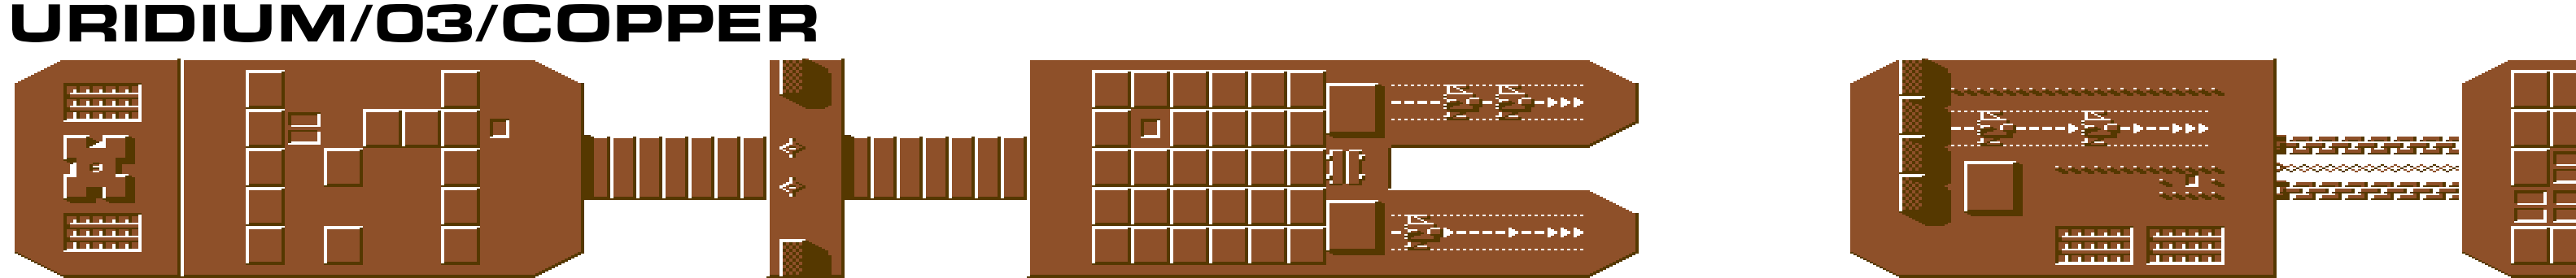
\includegraphics{src/surface_diagrams/3_horizontal_1.png}%
    \end{adjustbox}
\end{figure}
\begin{figure}[H]
    \begin{adjustbox}{height=1.8cm,left}
      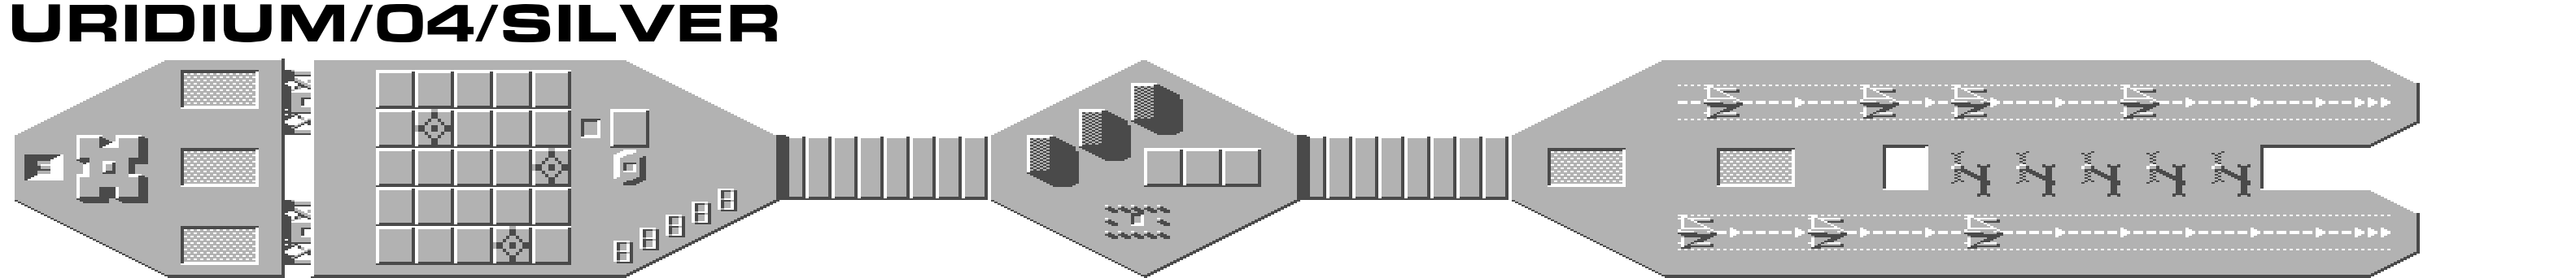
\includegraphics{src/surface_diagrams/4_horizontal_1.png}%
    \end{adjustbox}
\end{figure}
\vspace{-0.1cm}
\begin{figure}[H]
    \begin{adjustbox}{height=1.79cm,left}
      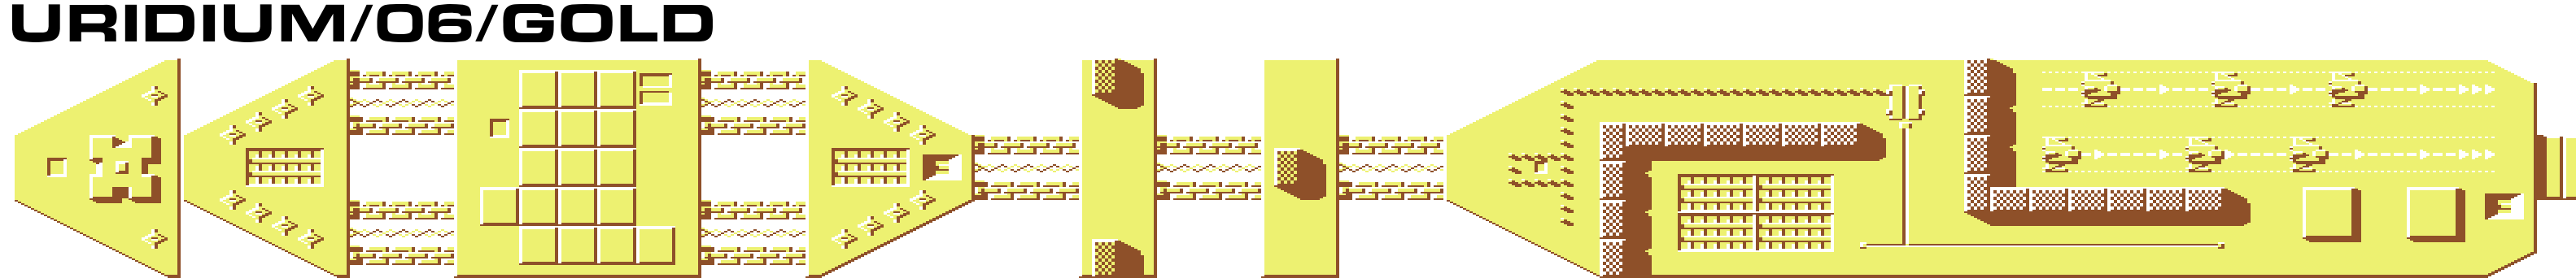
\includegraphics{src/surface_diagrams/6_horizontal_1.png}%
    \end{adjustbox}
\end{figure}
\vspace{-0.1cm}
\begin{figure}[H]
    \begin{adjustbox}{height=1.79cm,left}
      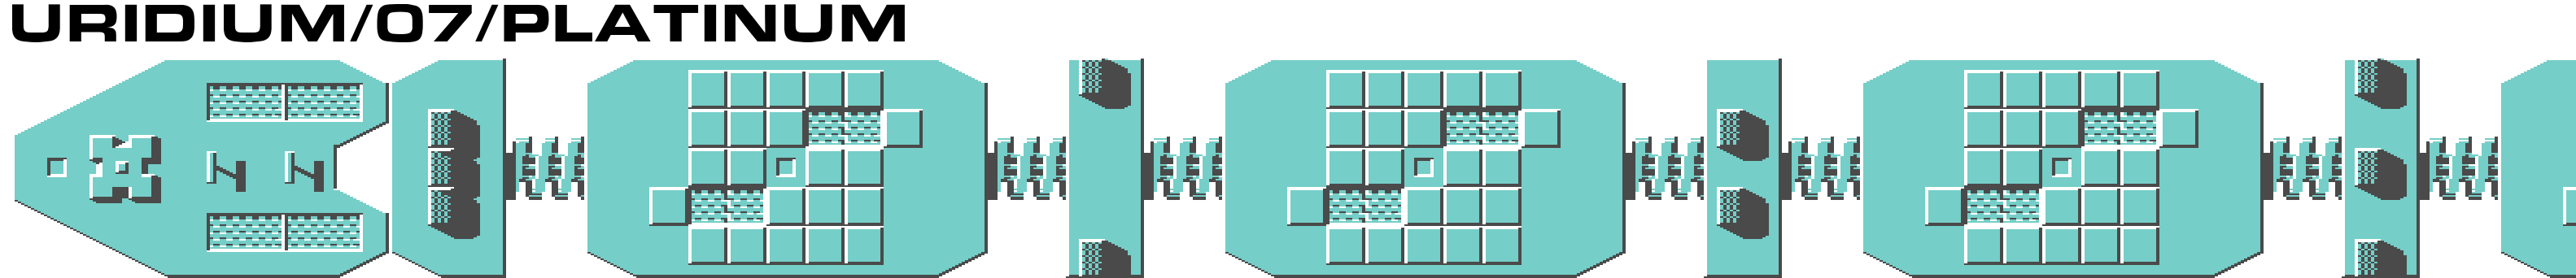
\includegraphics{src/surface_diagrams/7_horizontal_1.png}%
    \end{adjustbox}
\end{figure}
\vspace{-0.1cm}
\begin{figure}[H]
    \begin{adjustbox}{height=1.79cm,left}
      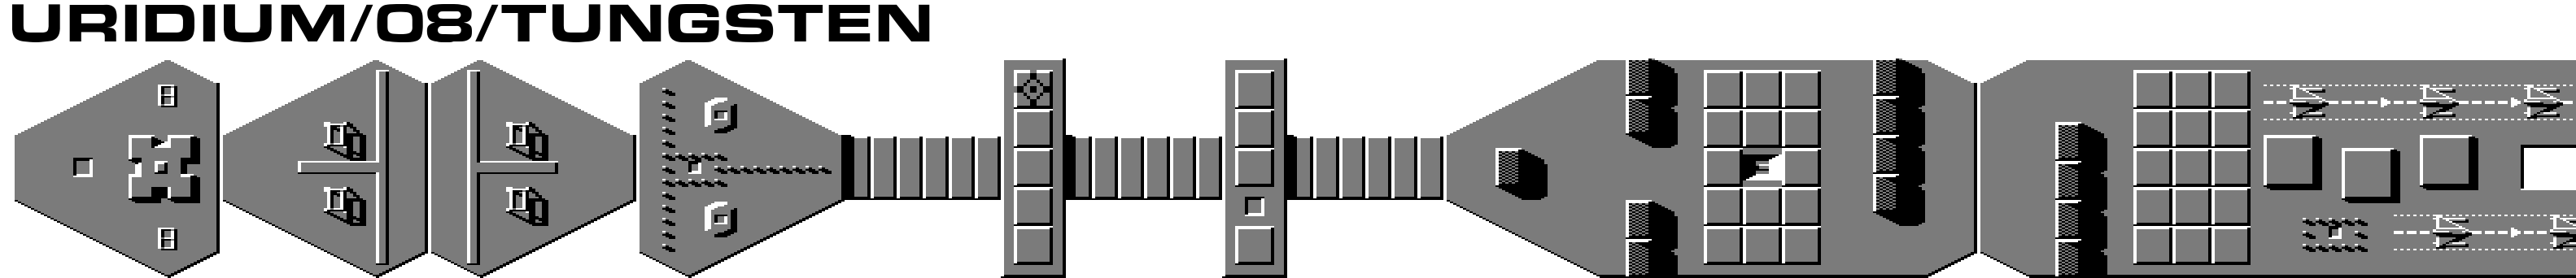
\includegraphics{src/surface_diagrams/8_horizontal_1.png}%
    \end{adjustbox}
\end{figure}
\clearpage

\begin{figure}[H]
    \hspace{0.92cm}
    \begin{adjustbox}{height=1.8cm,right}
      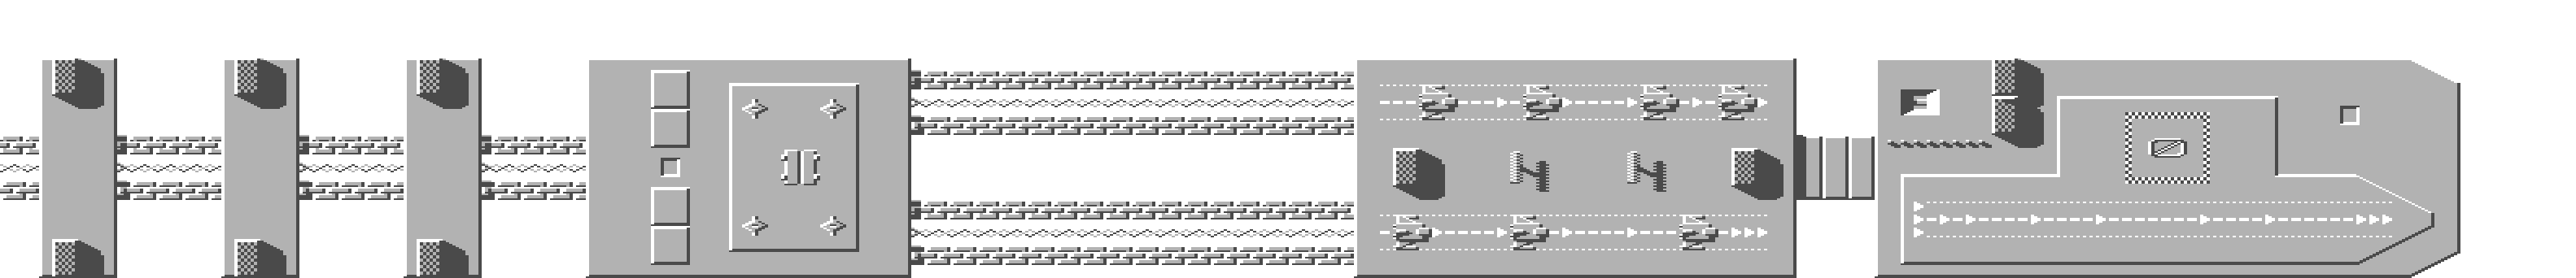
\includegraphics{src/surface_diagrams/1_horizontal_2.png}%
    \end{adjustbox}
\end{figure}
\vspace{-0.195cm}
\begin{figure}[H]
    \hspace{1.41cm}
    \begin{adjustbox}{height=1.8cm,right}
      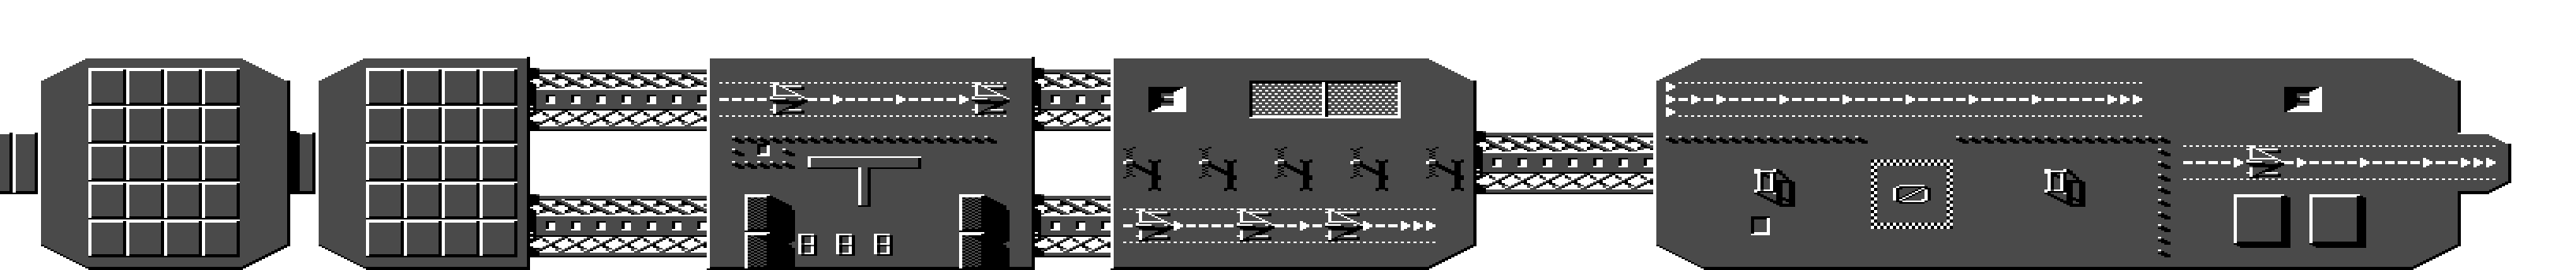
\includegraphics{src/surface_diagrams/2_horizontal_2.png}%
    \end{adjustbox}
\end{figure}
\vspace{-0.110cm}
\begin{figure}[H]
    \hspace{0.79cm}
    \begin{adjustbox}{height=1.79cm,right}
      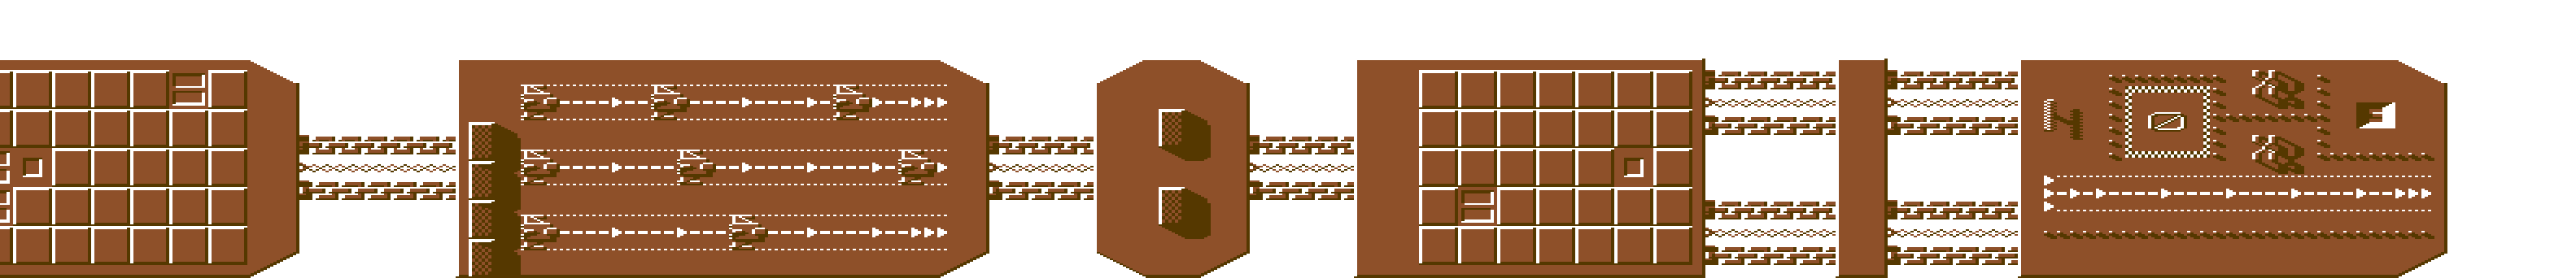
\includegraphics{src/surface_diagrams/3_horizontal_2.png}%
    \end{adjustbox}
\end{figure}
\begin{figure}[H]
    \hspace{0.92cm}
    \begin{adjustbox}{height=1.8cm,right}
      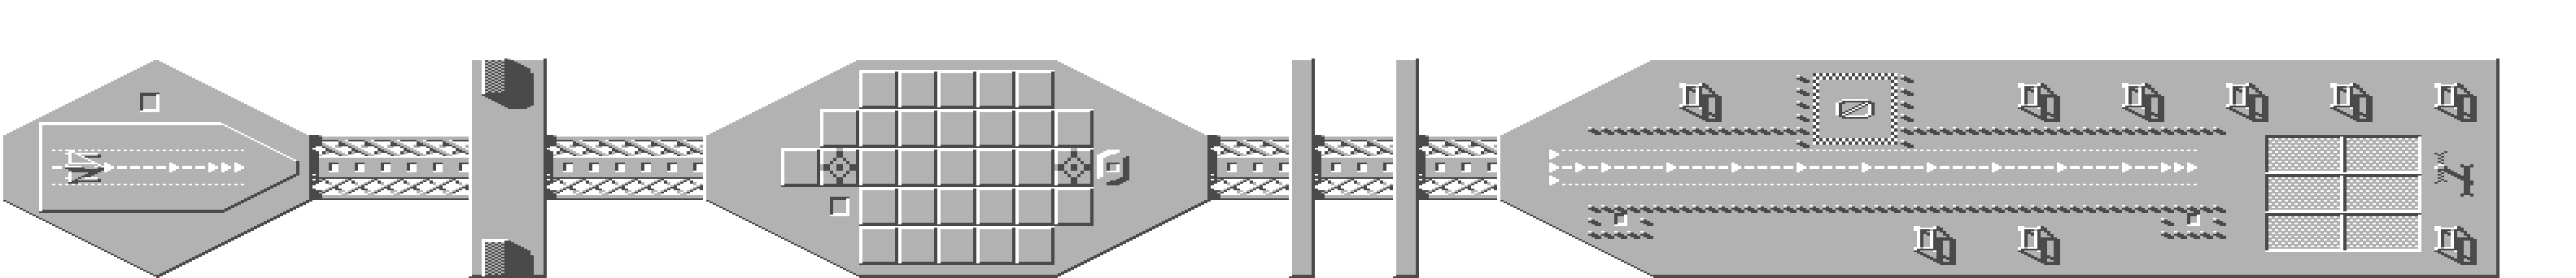
\includegraphics{src/surface_diagrams/4_horizontal_2.png}%
    \end{adjustbox}
\end{figure}
\vspace{-0.110cm}
\begin{figure}[H]
    \hspace{0.79cm}
    \begin{adjustbox}{height=1.79cm,right}
      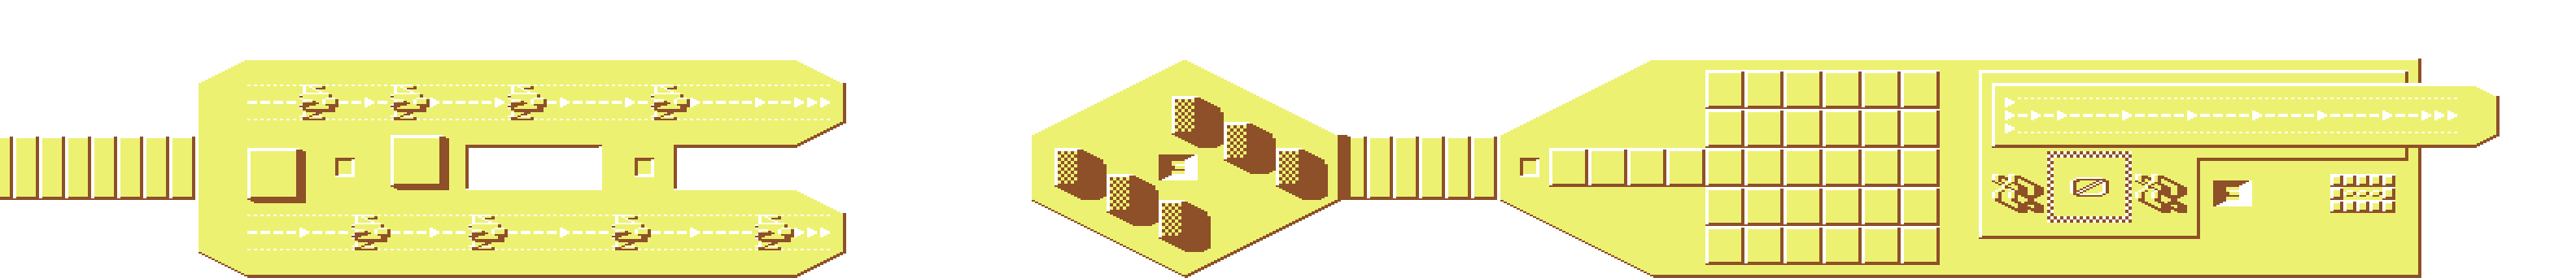
\includegraphics{src/surface_diagrams/6_horizontal_2.png}%
    \end{adjustbox}
\end{figure}
\vspace{-0.110cm}
\begin{figure}[H]
    \hspace{0.79cm}
    \begin{adjustbox}{height=1.79cm,right}
      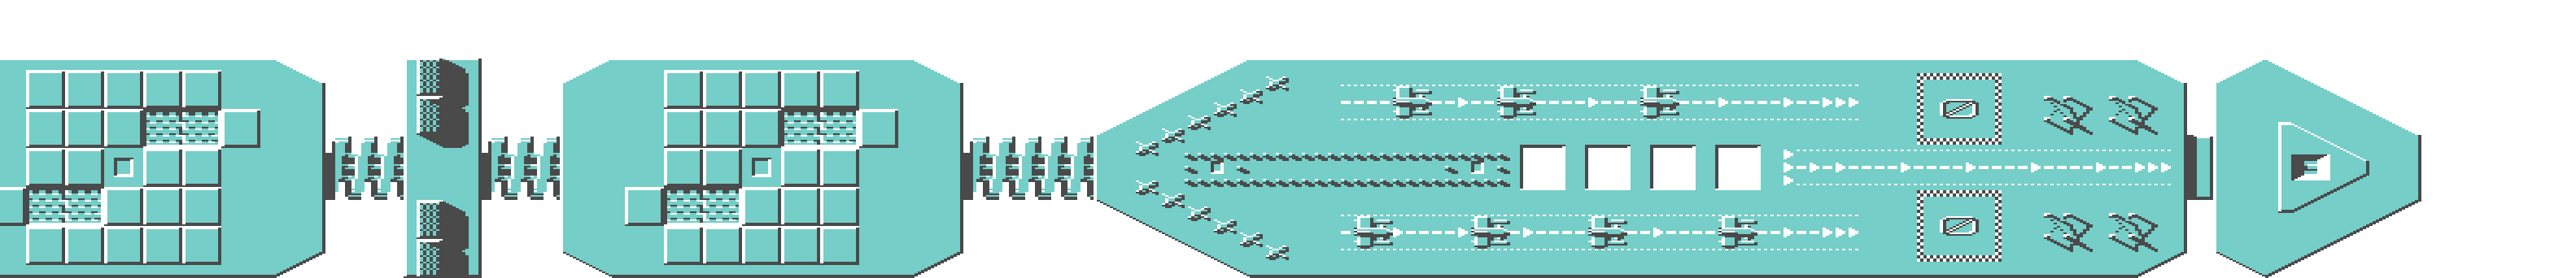
\includegraphics{src/surface_diagrams/7_horizontal_2.png}%
    \end{adjustbox}
\end{figure}
\vspace{-0.110cm}
\begin{figure}[H]
    \hspace{0.79cm}
    \begin{adjustbox}{height=1.79cm,right}
      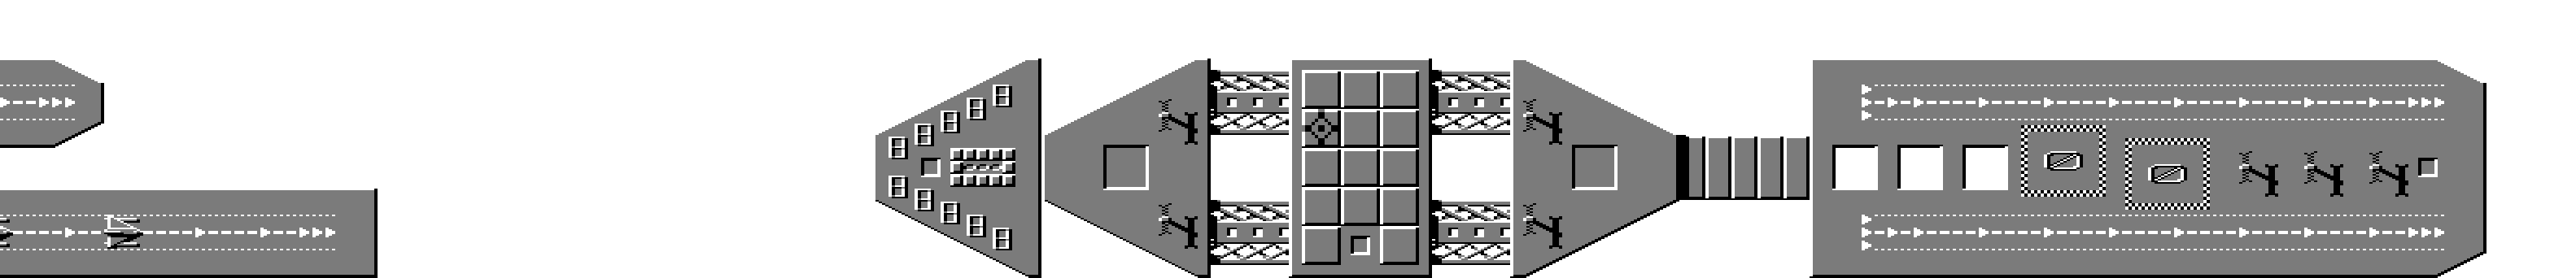
\includegraphics{src/surface_diagrams/8_horizontal_2.png}%
    \end{adjustbox}
\end{figure}
\clearpage

\clearpage
\begin{figure}[H]
    \begin{adjustbox}{height=1.8cm,left}
      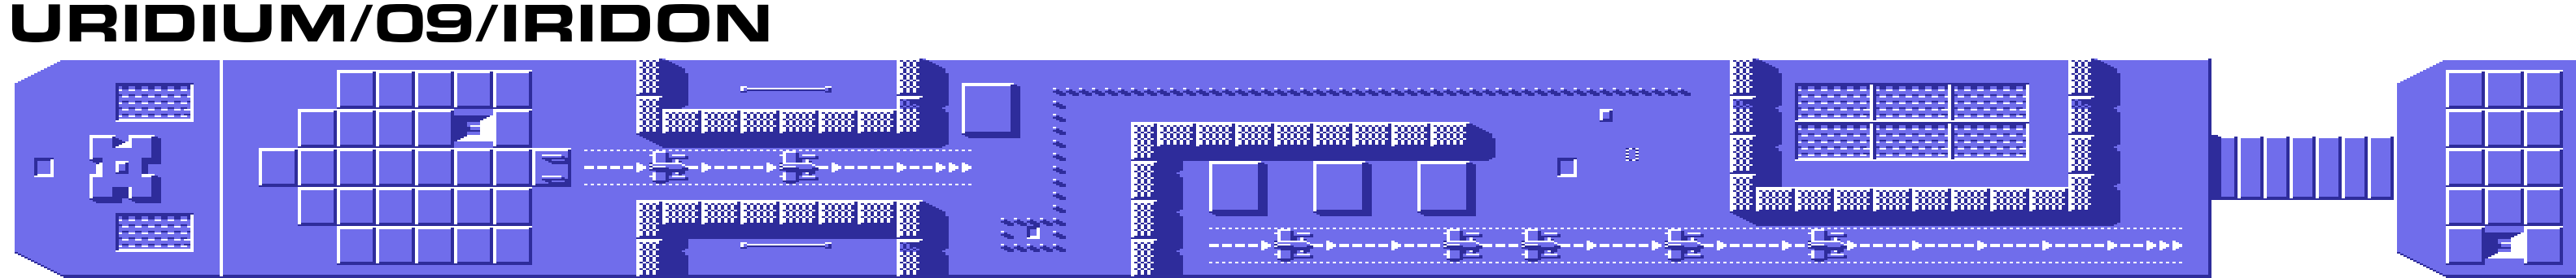
\includegraphics{src/surface_diagrams/9_horizontal_1.png}%
    \end{adjustbox}
\end{figure}
\vspace{-0.1cm}
\begin{figure}[H]
    \begin{adjustbox}{height=1.8cm,left}
      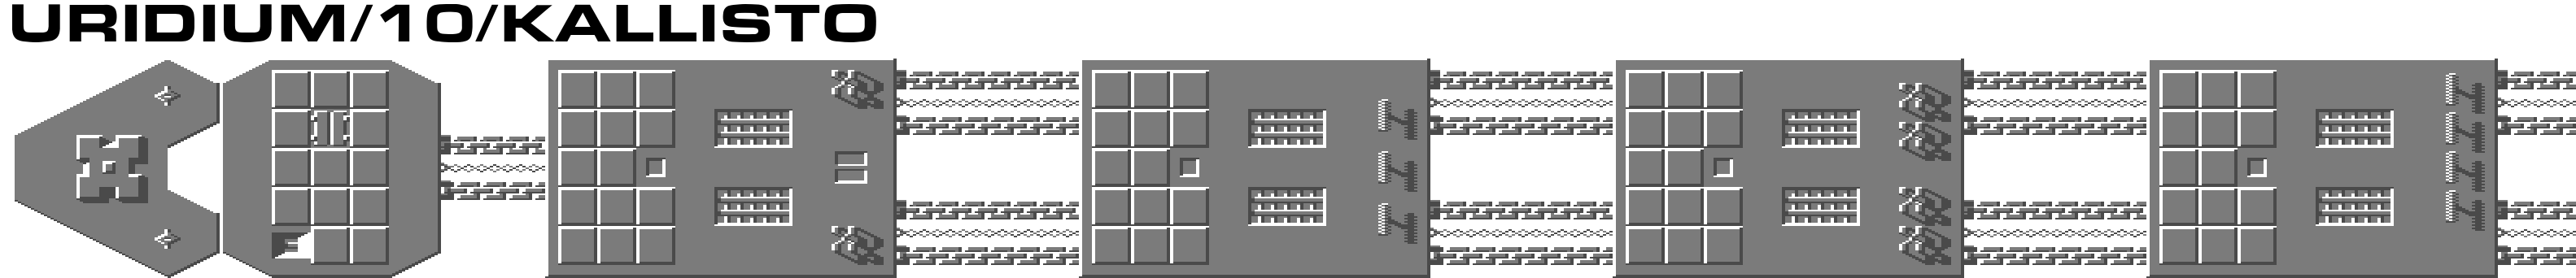
\includegraphics{src/surface_diagrams/10_horizontal_1.png}%
    \end{adjustbox}
\end{figure}
\vspace{-0.1cm}
\begin{figure}[H]
    \begin{adjustbox}{height=1.8cm,left}
      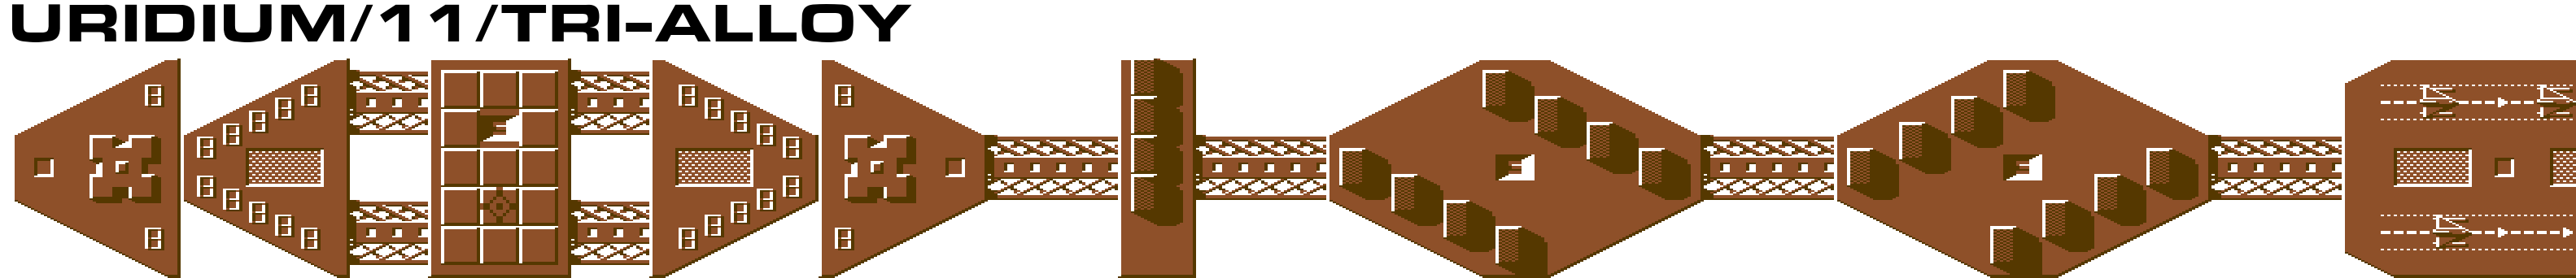
\includegraphics{src/surface_diagrams/11_horizontal_1.png}%
    \end{adjustbox}
\end{figure}
\vspace{-0.1cm}
\begin{figure}[H]
    \begin{adjustbox}{height=1.79cm,left}
      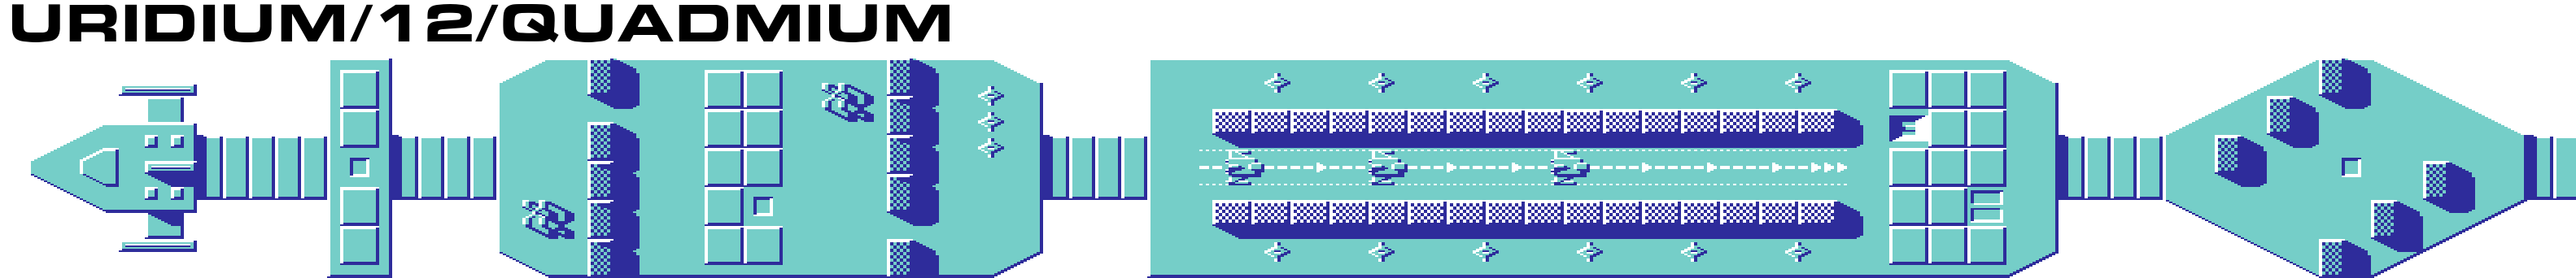
\includegraphics{src/surface_diagrams/12_horizontal_1.png}%
    \end{adjustbox}
\end{figure}
\begin{figure}[H]
    \begin{adjustbox}{height=1.8cm,left}
      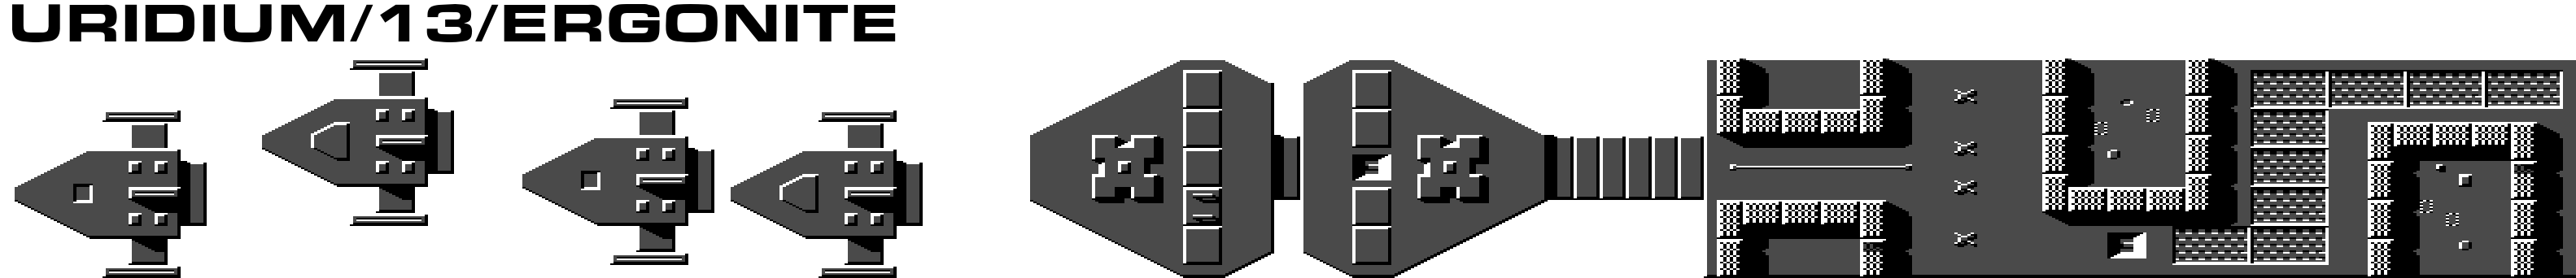
\includegraphics{src/surface_diagrams/13_horizontal_1.png}%
    \end{adjustbox}
\end{figure}
\vspace{-0.1cm}
\begin{figure}[H]
    \begin{adjustbox}{height=1.79cm,left}
      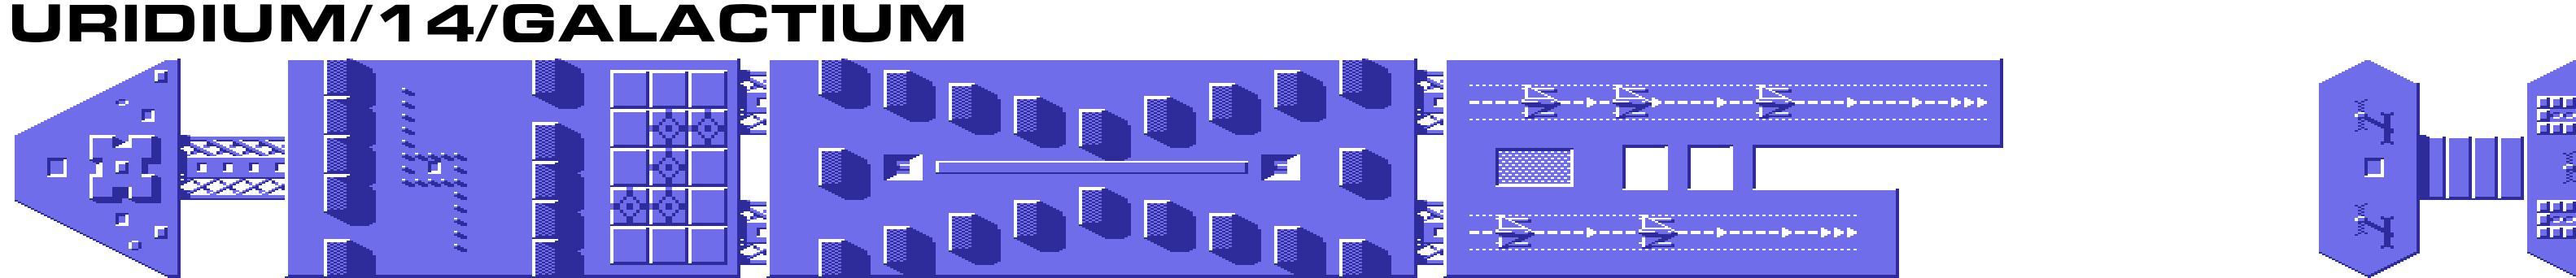
\includegraphics{src/surface_diagrams/14_horizontal_1.png}%
    \end{adjustbox}
\end{figure}
\vspace{-0.1cm}
\begin{figure}[H]
    \begin{adjustbox}{height=1.79cm,left}
      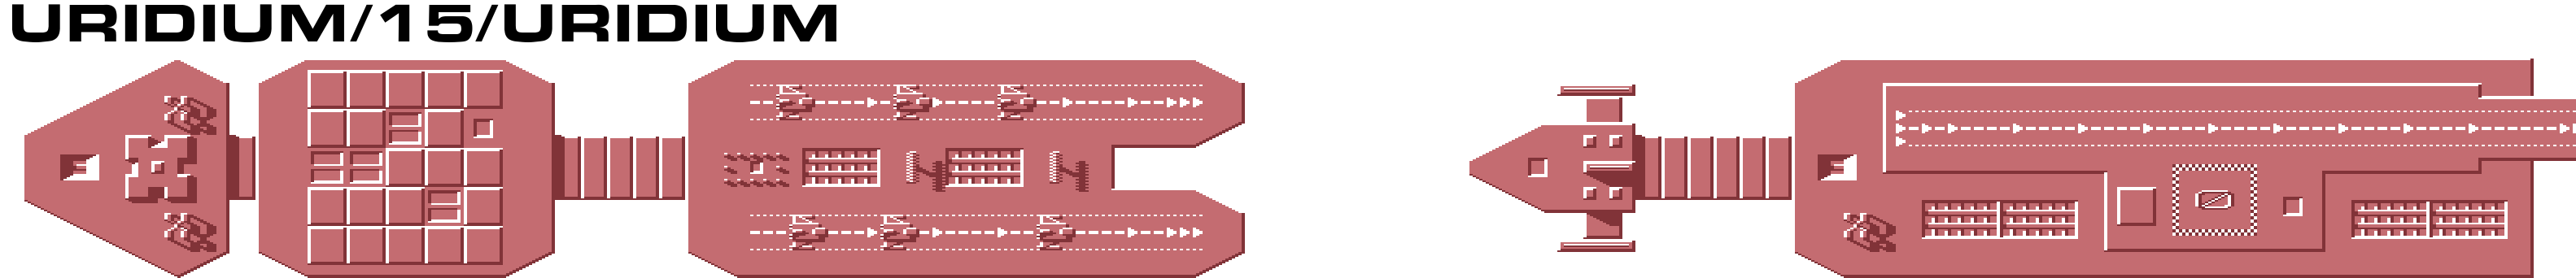
\includegraphics{src/surface_diagrams/15_horizontal_1.png}%
    \end{adjustbox}
\end{figure}
\clearpage

\begin{figure}[H]
    \hspace{0.92cm}
    \begin{adjustbox}{height=1.8cm,right}
      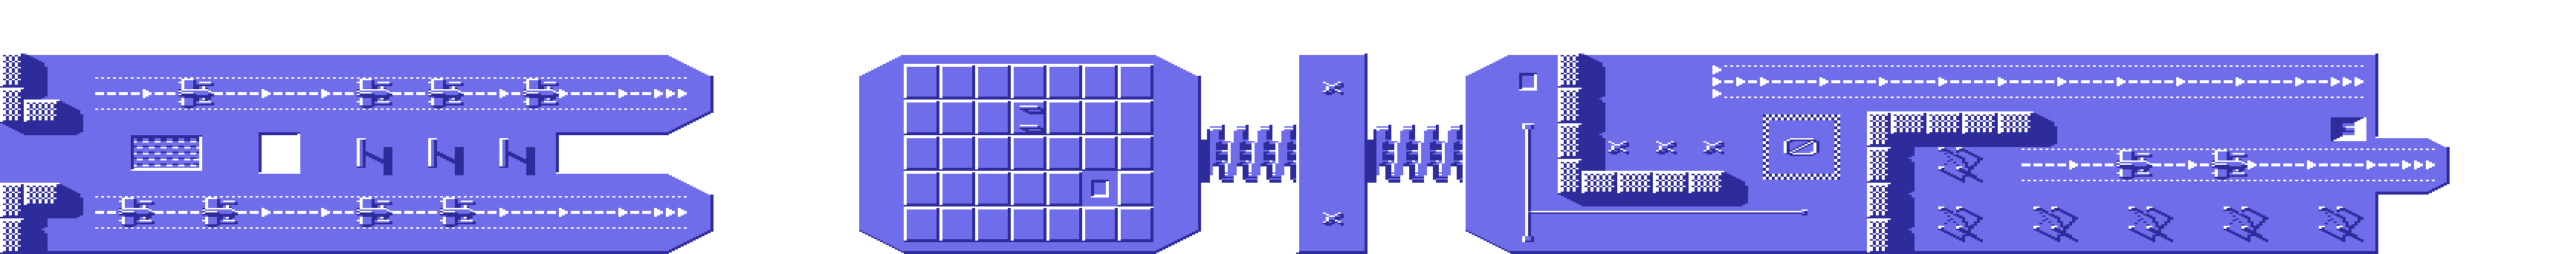
\includegraphics{src/surface_diagrams/9_horizontal_2.png}%
    \end{adjustbox}
\end{figure}
\vspace{-0.195cm}
\begin{figure}[H]
    \hspace{0.92cm}
    \begin{adjustbox}{height=1.8cm,right}
      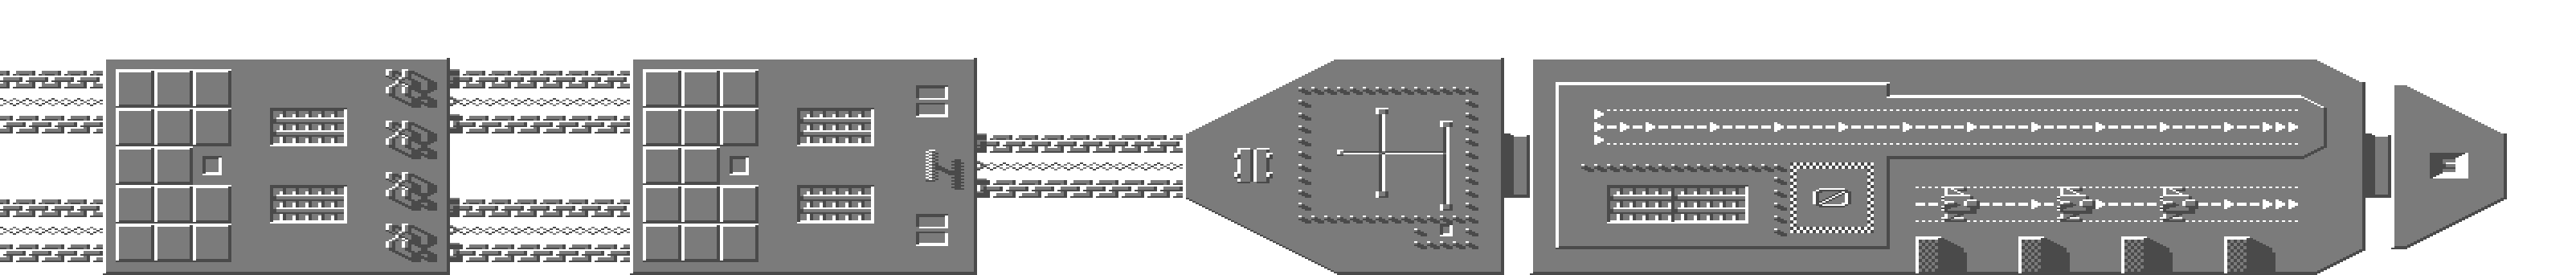
\includegraphics{src/surface_diagrams/10_horizontal_2.png}%
    \end{adjustbox}
\end{figure}
\vspace{-0.195cm}
\begin{figure}[H]
    \hspace{1.41cm}
    \begin{adjustbox}{height=1.8cm,right}
      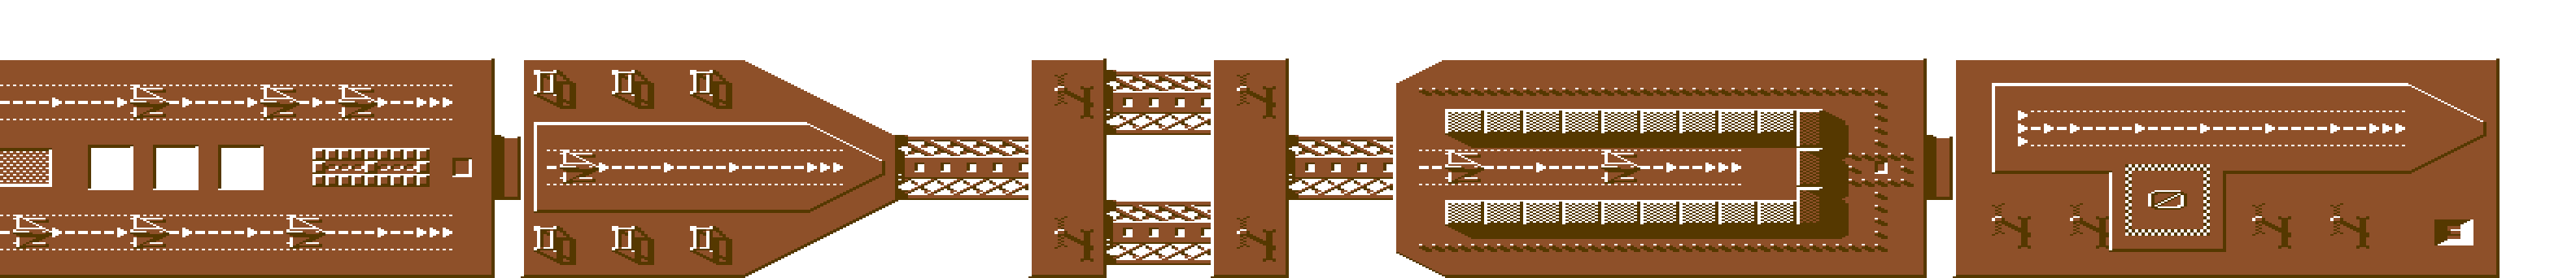
\includegraphics{src/surface_diagrams/11_horizontal_2.png}%
    \end{adjustbox}
\end{figure}
\vspace{-0.110cm}
\begin{figure}[H]
    \hspace{0.79cm}
    \begin{adjustbox}{height=1.79cm,right}
      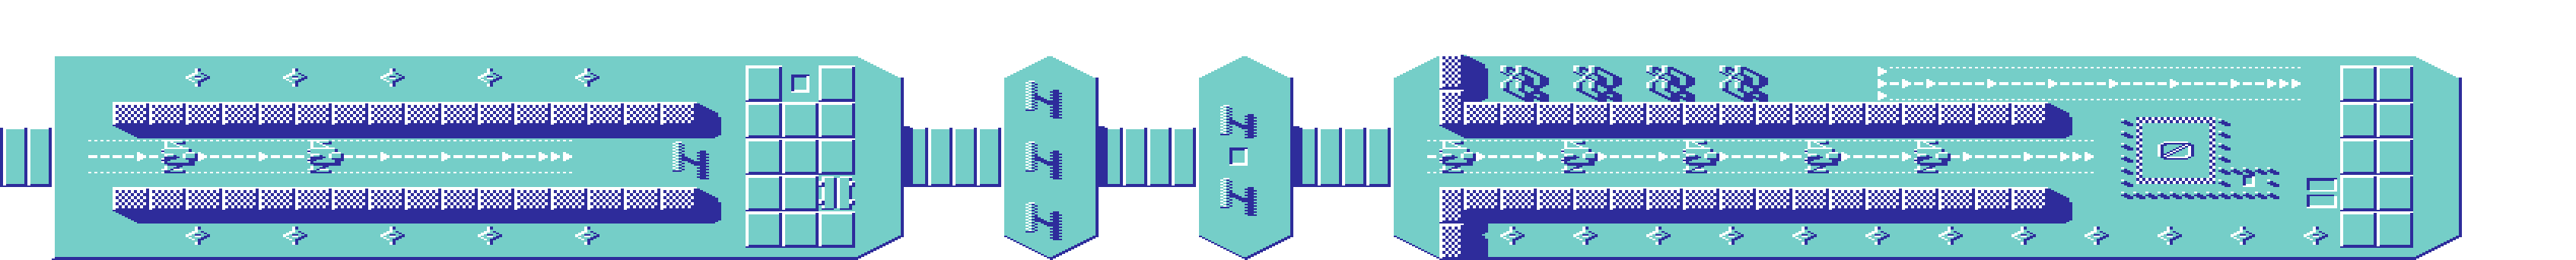
\includegraphics{src/surface_diagrams/12_horizontal_2.png}%
    \end{adjustbox}
\end{figure}
\begin{figure}[H]
    \hspace{0.92cm}
    \begin{adjustbox}{height=1.8cm,right}
      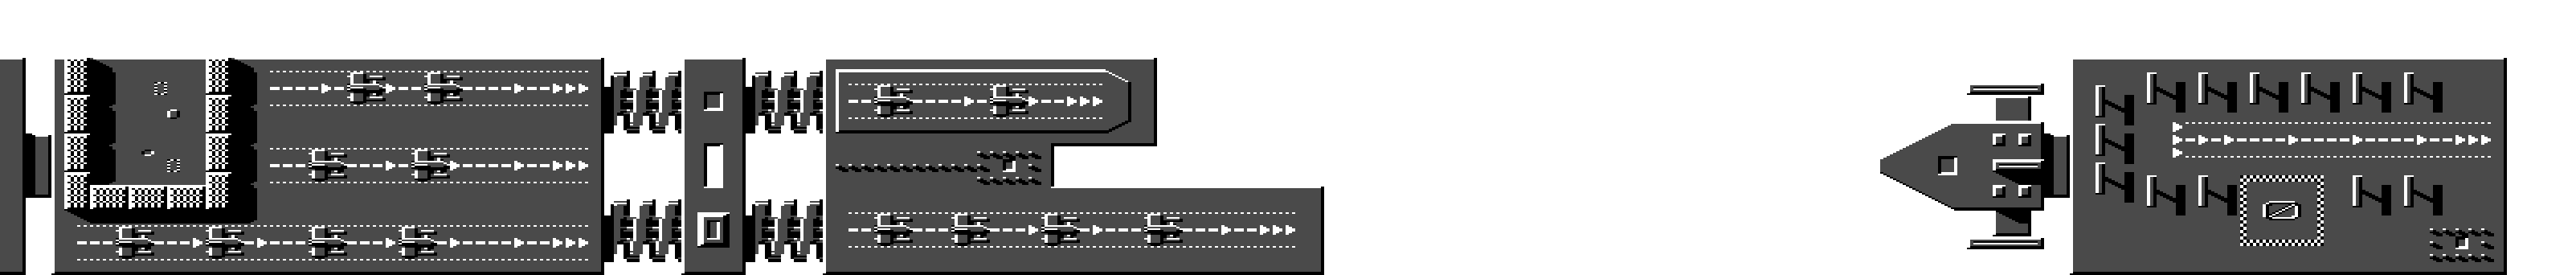
\includegraphics{src/surface_diagrams/13_horizontal_2.png}%
    \end{adjustbox}
\end{figure}
\vspace{-0.110cm}
\begin{figure}[H]
    \hspace{0.79cm}
    \begin{adjustbox}{height=1.79cm,right}
      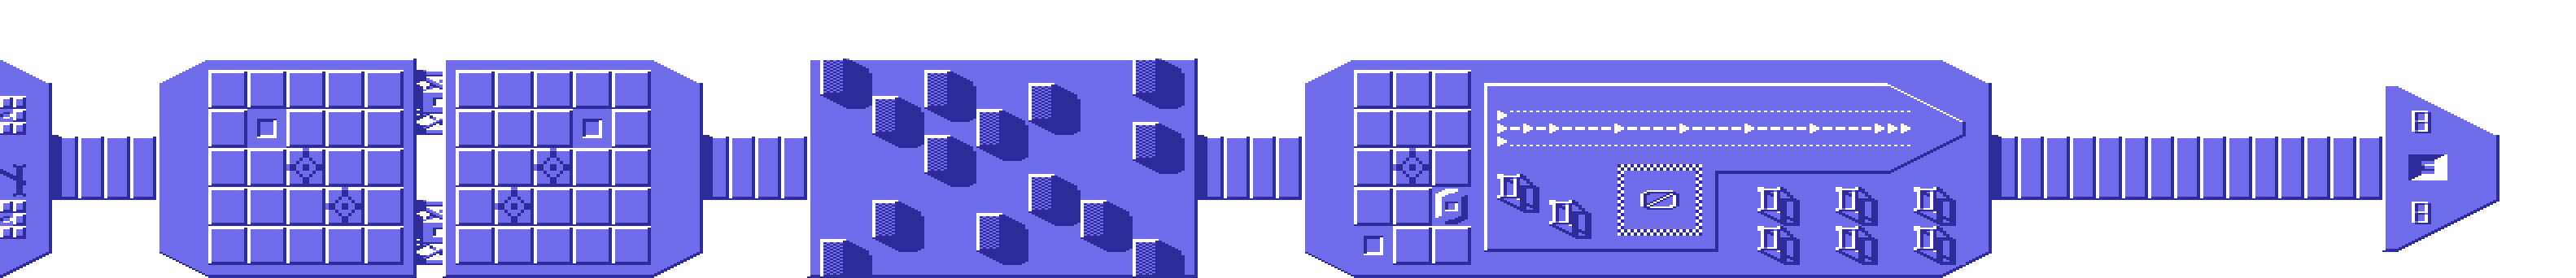
\includegraphics{src/surface_diagrams/14_horizontal_2.png}%
    \end{adjustbox}
\end{figure}
\vspace{-0.110cm}
\begin{figure}[H]
    \hspace{0.79cm}
    \begin{adjustbox}{height=1.79cm,right}
      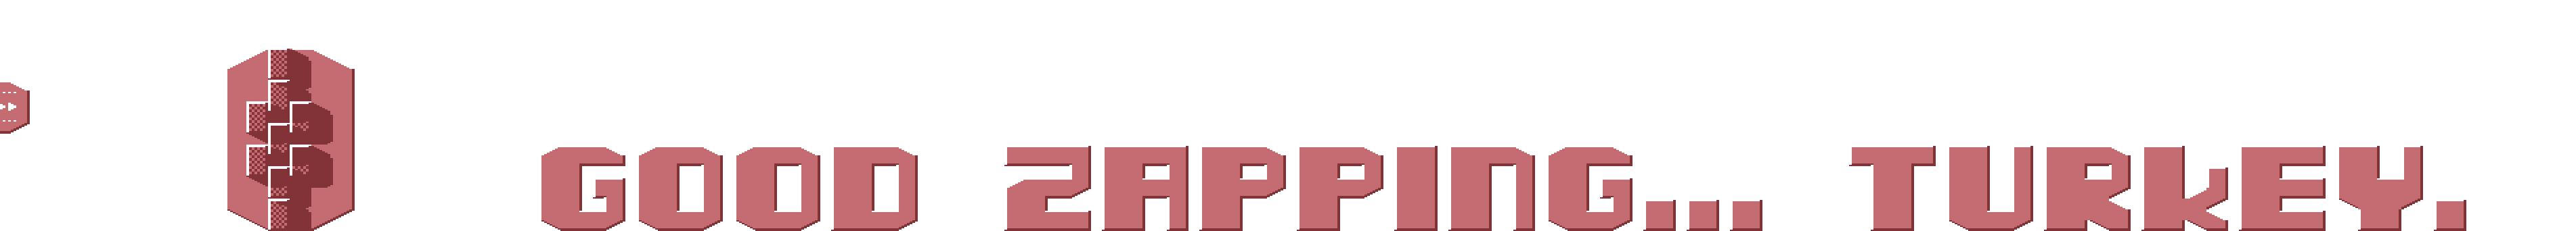
\includegraphics{src/surface_diagrams/15_horizontal_2.png}%
    \end{adjustbox}
\end{figure}
\clearpage

\vspace{-0.6cm}
\begin{figure}[H]
    \begin{adjustbox}{height=1.8cm,left}
      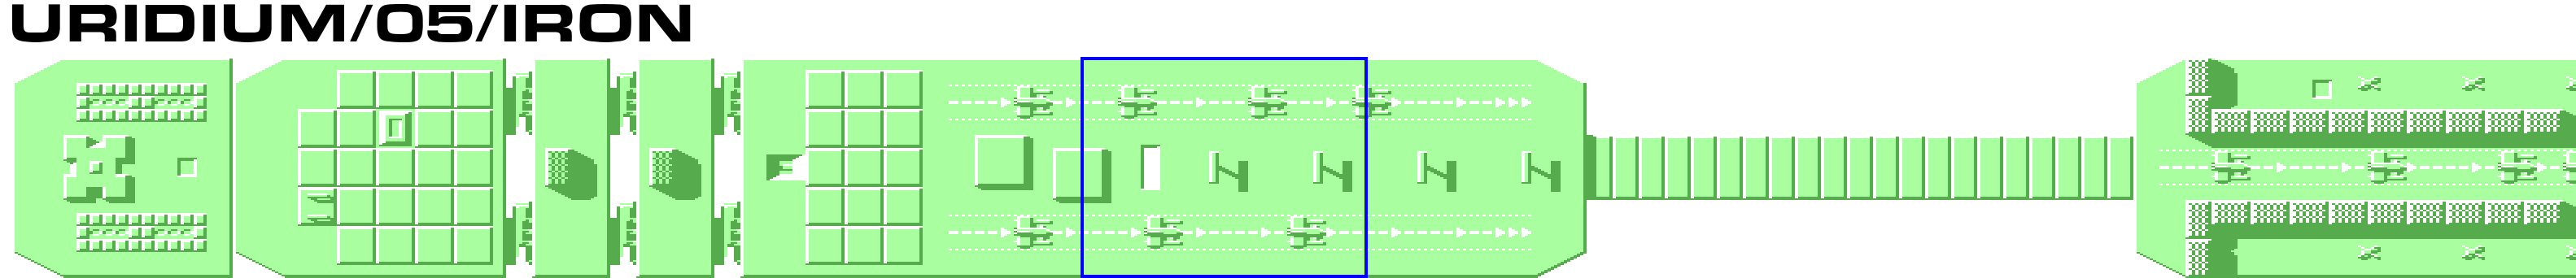
\includegraphics{src/surface_diagrams/5_horizontal_1_highlight.png}%
    \end{adjustbox}
\end{figure}
\vspace{-0.4cm}

If we zoom in on a section of one of the dreadnoughts (the blue inset above) we can get a sense of
the constituent parts of the whole.
\begin{figure}[H]
    \centering
    \begin{adjustbox}{width=14cm,center}
      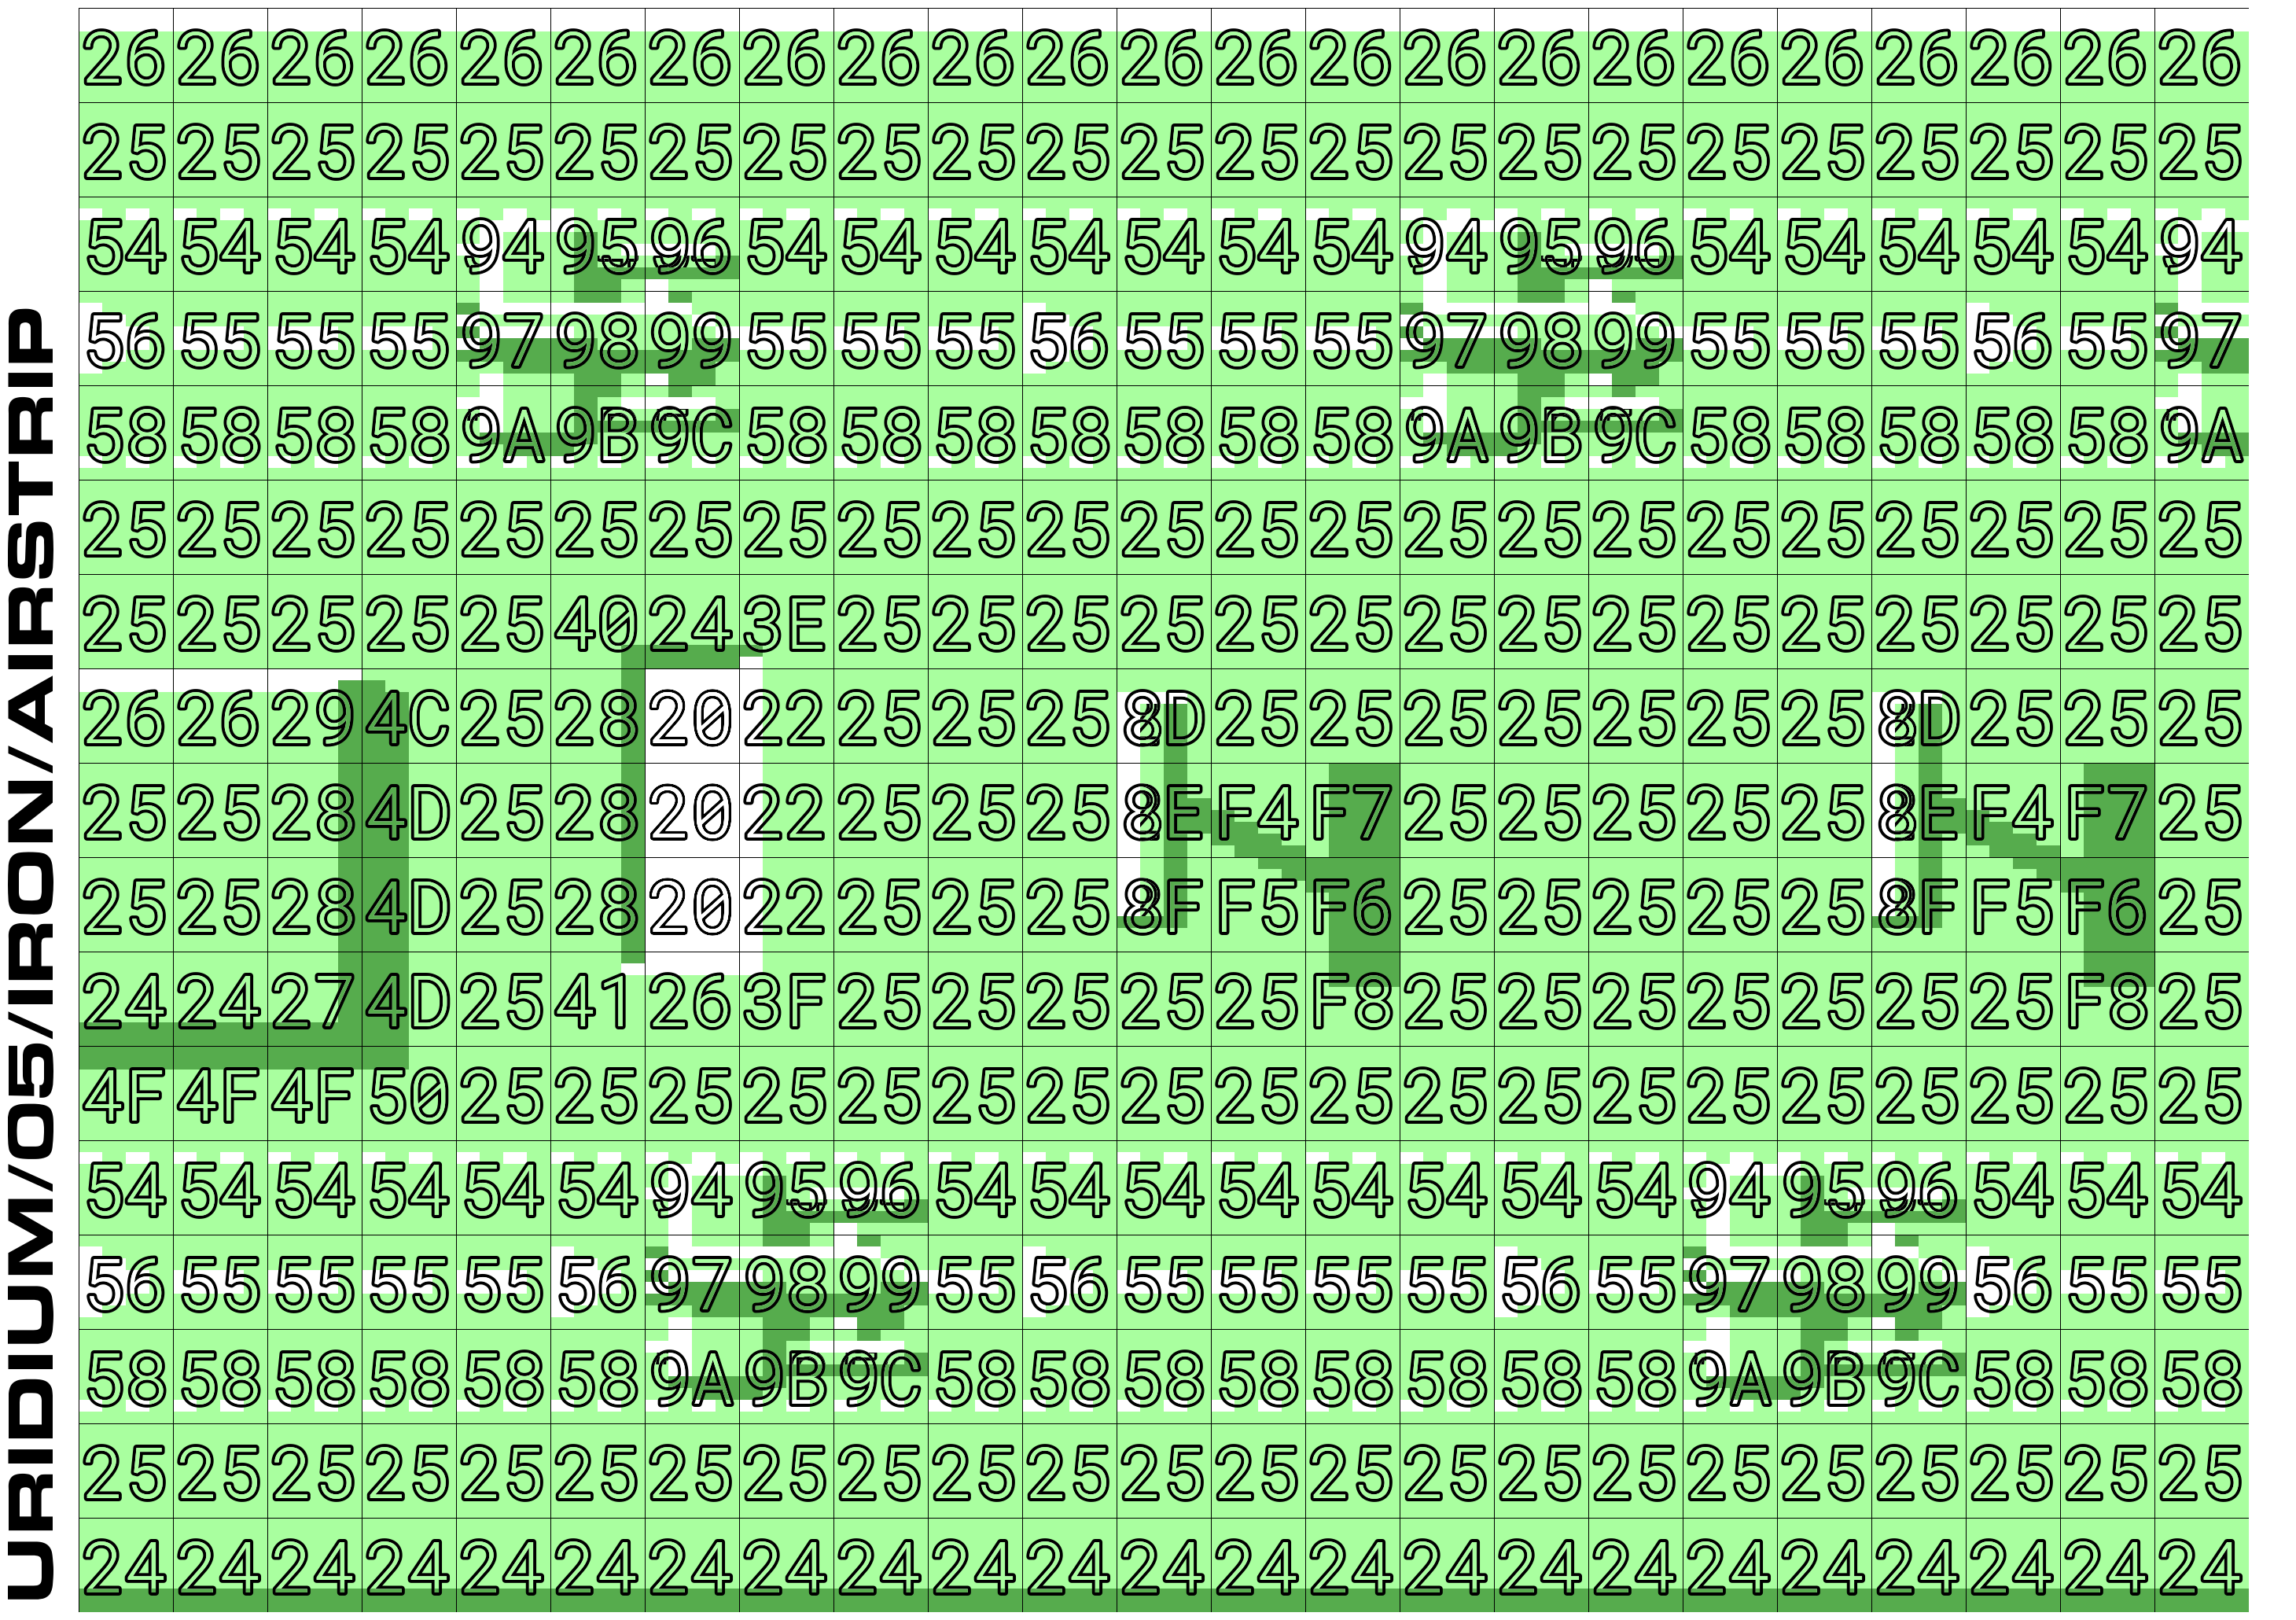
\includegraphics[width=15cm]{src/section_diagrams/5_AIRSTRIP.png}%
    \end{adjustbox}
\end{figure}
\vspace{-0.4cm}
What we find is that the dreadnought is composed of small square tiles. Each type of tile has its own
identifier, or index number, and with these we can build a complete dreadnought, fitting them together
as appropriate. In total each dreadnought can be up to 512 tiles wide and 17 tiles high, giving a total
quantity of 8704 tiles required to create an entire ship. Our indexing scheme allows up to 255 different types of tiles so we are not short of the potential
for complexity. In just the section we have extracted above we have used 28 different tiles.


\clearpage
\vspace{-0.595cm}
\begin{figure}[H]
    \hspace{0.41cm}
    \begin{adjustbox}{height=1.8cm,right}
      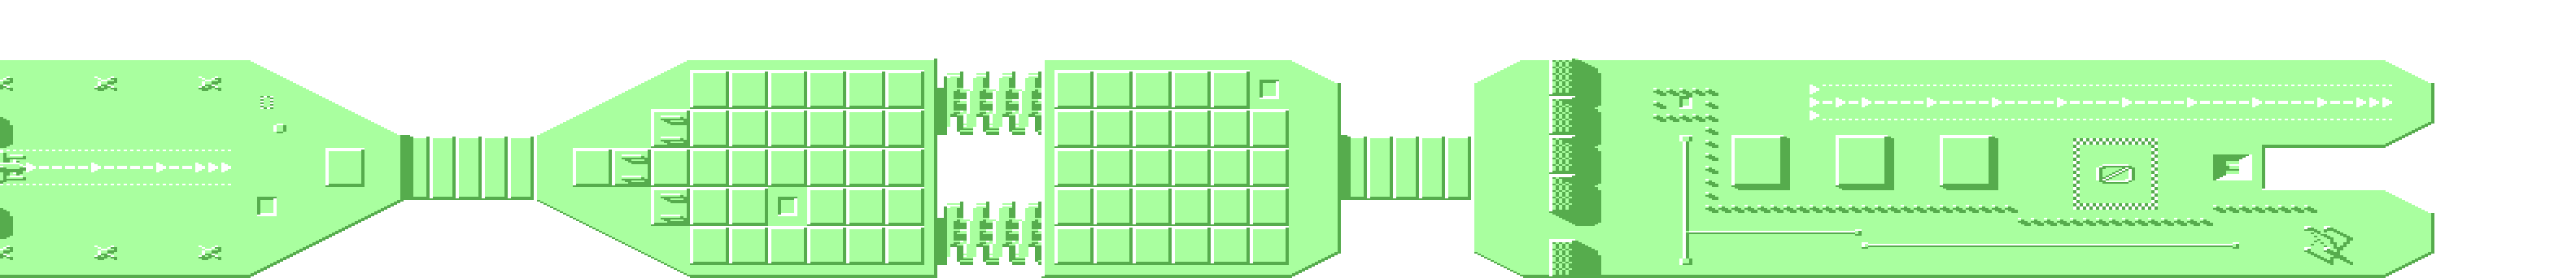
\includegraphics{src/surface_diagrams/5_horizontal_2.png}%
    \end{adjustbox}
\end{figure}
\vspace{-0.4cm}

It is easier to see what the individual tiles look like if we set them out individually. Here they are,
in descending order of frequency with which they appear in our diagram:

\begin{figure}[H]
    \centering
\raisebox{-0.3\totalheight}{
\includegraphics[height=1.0cm]{src/surface_character_mini_diagrams/5_25.png}}
\hspace{0.1cm}
\raisebox{-0.3\totalheight}{
\includegraphics[height=1.0cm]{src/surface_character_mini_diagrams/5_26.png}}
\hspace{0.1cm}
\raisebox{-0.3\totalheight}{
\includegraphics[height=1.0cm]{src/surface_character_mini_diagrams/5_54.png}}
\hspace{0.1cm}
\raisebox{-0.3\totalheight}{
\includegraphics[height=1.0cm]{src/surface_character_mini_diagrams/5_55.png}}
\hspace{0.1cm}
\raisebox{-0.3\totalheight}{
\includegraphics[height=1.0cm]{src/surface_character_mini_diagrams/5_58.png}}
\hspace{0.1cm}
\raisebox{-0.3\totalheight}{
\includegraphics[height=1.0cm]{src/surface_character_mini_diagrams/5_56.png}}
\hspace{0.1cm}
\raisebox{-0.3\totalheight}{
\includegraphics[height=1.0cm]{src/surface_character_mini_diagrams/5_24.png}}
\hspace{0.1cm}
\raisebox{-0.3\totalheight}{
\includegraphics[height=1.0cm]{src/surface_character_mini_diagrams/5_8D.png}}
\hspace{0.1cm}
\raisebox{-0.3\totalheight}{
\includegraphics[height=1.0cm]{src/surface_character_mini_diagrams/5_8E.png}}
\hspace{0.1cm}
\raisebox{-0.3\totalheight}{
\includegraphics[height=1.0cm]{src/surface_character_mini_diagrams/5_8F.png}}
\hspace{0.1cm}
\raisebox{-0.3\totalheight}{
\includegraphics[height=1.0cm]{src/surface_character_mini_diagrams/5_94.png}}
\hspace{0.1cm}
\raisebox{-0.3\totalheight}{
\includegraphics[height=1.0cm]{src/surface_character_mini_diagrams/5_95.png}}
\end{figure}
\vspace{-0.4cm}

\begin{figure}[H]
    \centering
\raisebox{-0.3\totalheight}{
\includegraphics[height=1.0cm]{src/surface_character_mini_diagrams/5_96.png}}
\hspace{0.1cm}
\raisebox{-0.3\totalheight}{
\includegraphics[height=1.0cm]{src/surface_character_mini_diagrams/5_97.png}}
\hspace{0.1cm}
\raisebox{-0.3\totalheight}{
\includegraphics[height=1.0cm]{src/surface_character_mini_diagrams/5_98.png}}
\hspace{0.1cm}
\raisebox{-0.3\totalheight}{
\includegraphics[height=1.0cm]{src/surface_character_mini_diagrams/5_99.png}}
\hspace{0.1cm}
\raisebox{-0.3\totalheight}{
\includegraphics[height=1.0cm]{src/surface_character_mini_diagrams/5_9A.png}}
\hspace{0.1cm}
\raisebox{-0.3\totalheight}{
\includegraphics[height=1.0cm]{src/surface_character_mini_diagrams/5_9B.png}}
\hspace{0.1cm}
\raisebox{-0.3\totalheight}{
\includegraphics[height=1.0cm]{src/surface_character_mini_diagrams/5_9C.png}}
\hspace{0.1cm}
\raisebox{-0.3\totalheight}{
\includegraphics[height=1.0cm]{src/surface_character_mini_diagrams/5_F4.png}}
\hspace{0.1cm}
\raisebox{-0.3\totalheight}{
\includegraphics[height=1.0cm]{src/surface_character_mini_diagrams/5_F5.png}}
\hspace{0.1cm}
\raisebox{-0.3\totalheight}{
\includegraphics[height=1.0cm]{src/surface_character_mini_diagrams/5_F6.png}}
\hspace{0.1cm}
\raisebox{-0.3\totalheight}{
\includegraphics[height=1.0cm]{src/surface_character_mini_diagrams/5_F7.png}}
\hspace{0.1cm}
\raisebox{-0.3\totalheight}{
\includegraphics[height=1.0cm]{src/surface_character_mini_diagrams/5_4F.png}}
\end{figure}
\vspace{-0.4cm}

We are clearly dealing with abstract forms that only make sense when composed together. Looking more
closely at the diagram opposite we can apprehend a distinction between two different ways in which the
tiles are used to render the dreadnought. The first is that low-numbered tiles tend to be used to draw
the surface areas of the ship. The second is that relatively high-numbered tiles are used to form the
structures that are dotted across it. This distinction will prove important in the following two chapters
when we look at the way the game stores and constructs the dreadnoughts.

Before we do that though, there is yet another level of granularity to which we can zoom down. This is the
detail required to render each of the constituent tiles. Each tile is defined by an array of eight bytes.
This scheme is very similar to the one used for sprites but instead defines a graphical element that is
eight pixels wide by eight pixels high. Putting tiles \icode{24} and \icode{8D} side by side we get a sense
of how each color unit is defined by a bitpair, giving us a tile that is four color units wide and eight
color units tall.

\begin{figure}[H]
    \centering
\raisebox{-0.3\totalheight}{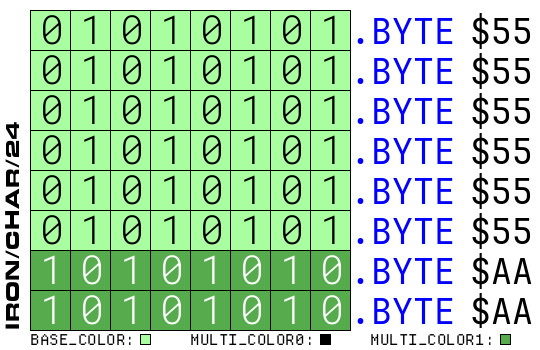
\includegraphics[width=6.3cm]{src/character_set_diagrams/5_24.png}}
\raisebox{-0.3\totalheight}{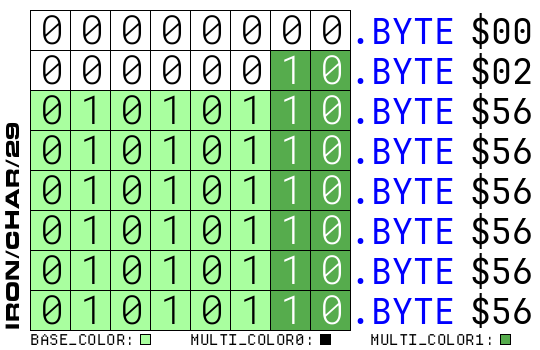
\includegraphics[width=6.3cm]{src/character_set_diagrams/5_29.png}}
\end{figure}
\vspace{-0.4cm}
\clearpage

\vspace{-0.6cm}
\begin{figure}[H]
    \begin{adjustbox}{height=1.8cm,left}
      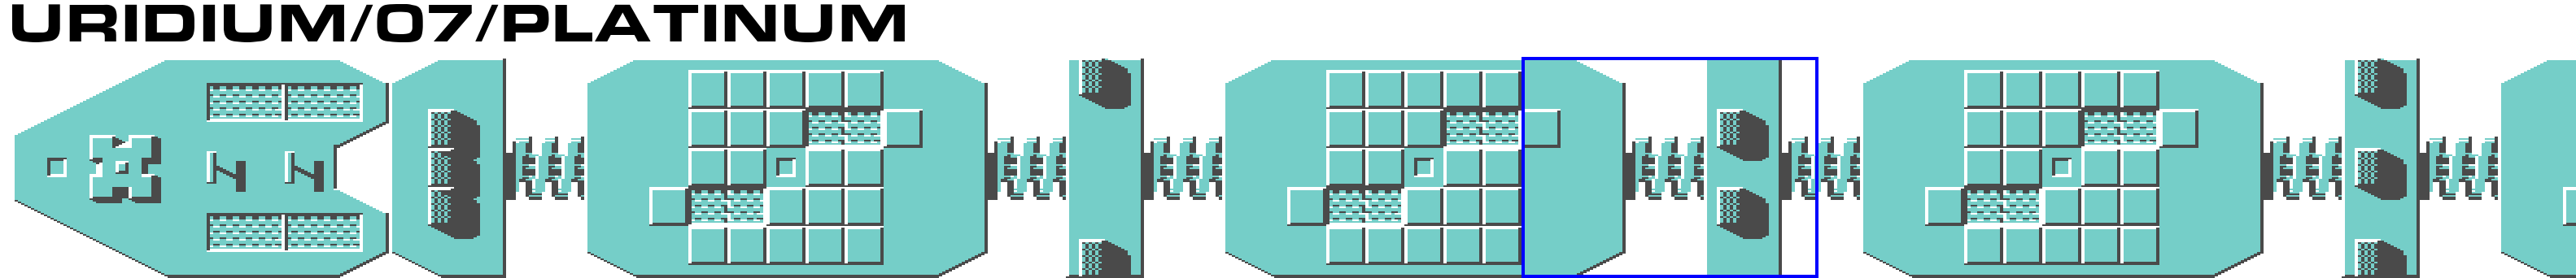
\includegraphics{src/surface_diagrams/7_horizontal_1_highlight.png}%
    \end{adjustbox}
\end{figure}
\vspace{-0.4cm}

Before we move on to examining how the surface of the dreadnought and its structures are stored and
constructed by the game, let's look at the segment of another level. This time it's the dreadnought
that makes up level 7. We focus in on a section of coupling that binds one carriage with another.
\begin{figure}[H]
    \centering
    \begin{adjustbox}{width=14cm,center}
      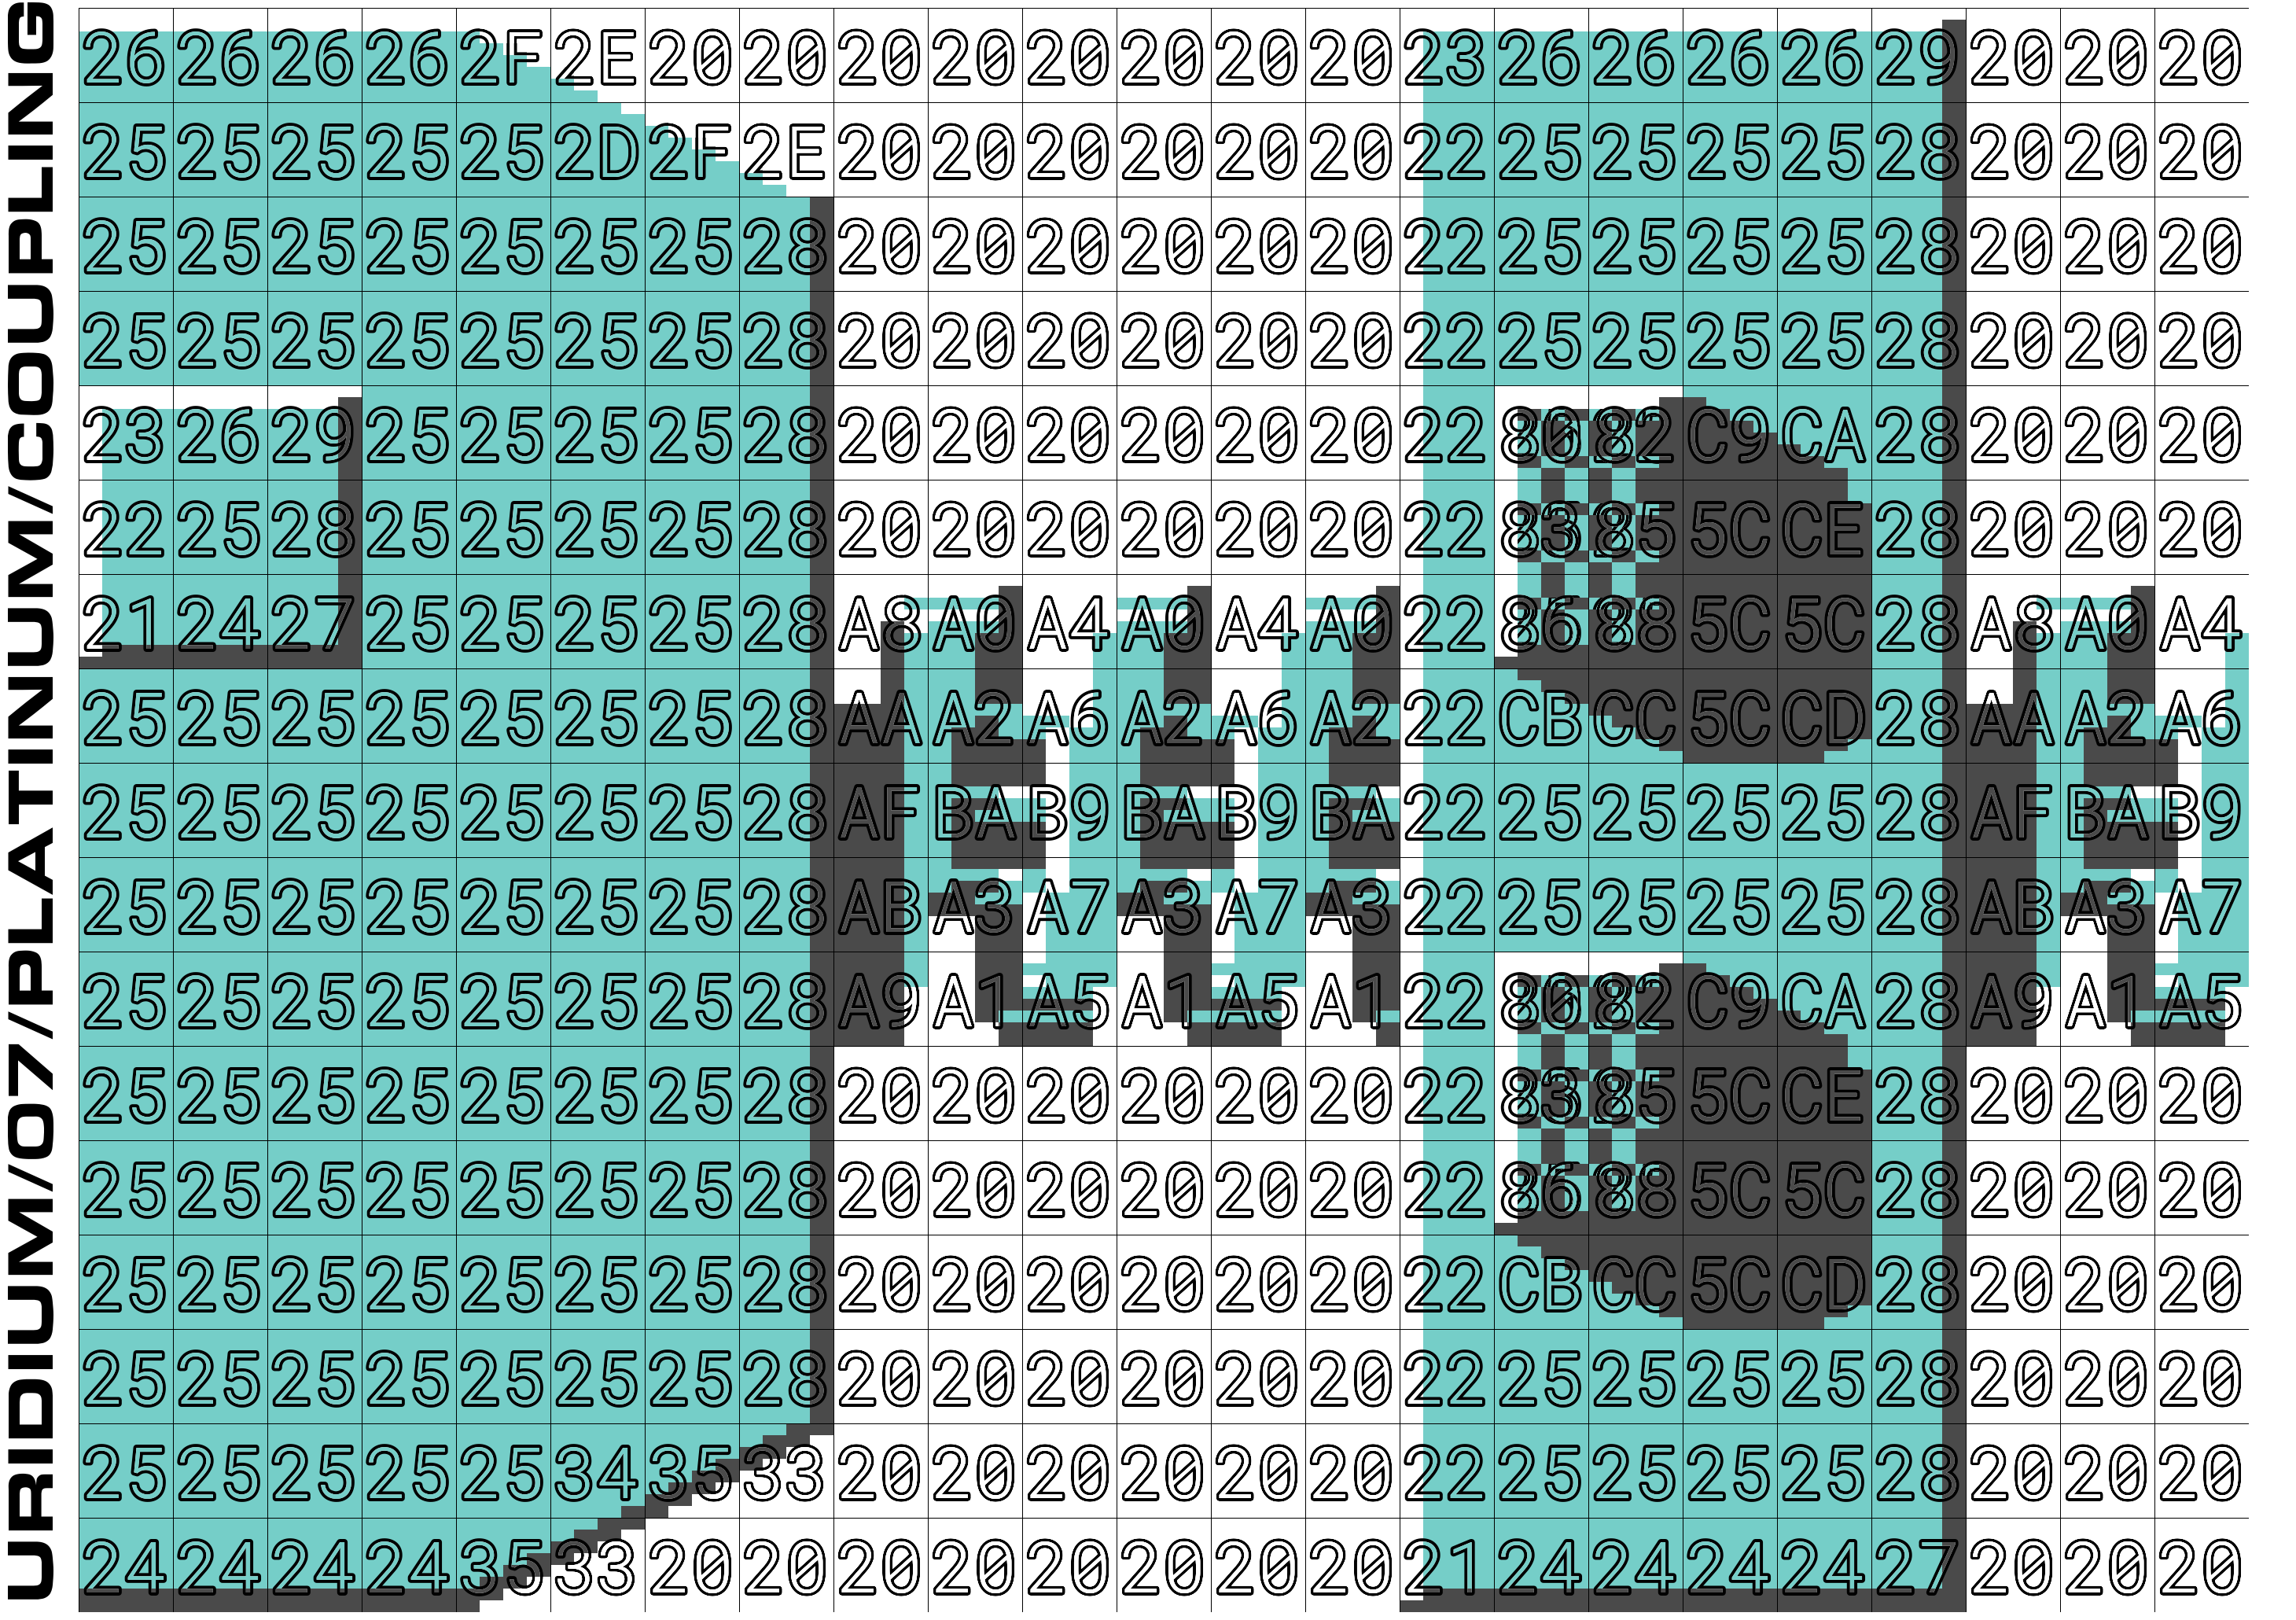
\includegraphics[width=15cm]{src/section_diagrams/7_COUPLING.png}%
    \end{adjustbox}
\end{figure}
\vspace{-0.4cm}
We find many of the tiles we are using here are the same as in the previous level, especially when
defining the surface of the dreadnought. 

\begin{figure}[H]
    \centering
\raisebox{-0.3\totalheight}{
\includegraphics[height=1.0cm]{src/surface_character_mini_diagrams/7_25.png}}
\hspace{0.1cm}
\raisebox{-0.3\totalheight}{
\includegraphics[height=1.0cm]{src/surface_character_mini_diagrams/7_26.png}}
\hspace{0.1cm}
\raisebox{-0.3\totalheight}{
\includegraphics[height=1.0cm]{src/surface_character_mini_diagrams/7_5C.png}}
\hspace{0.1cm}
\raisebox{-0.3\totalheight}{
\includegraphics[height=1.0cm]{src/surface_character_mini_diagrams/7_5D.png}}
\hspace{0.1cm}
\raisebox{-0.3\totalheight}{
\includegraphics[height=1.0cm]{src/surface_character_mini_diagrams/7_5E.png}}
\hspace{0.1cm}
\raisebox{-0.3\totalheight}{
\includegraphics[height=1.0cm]{src/surface_character_mini_diagrams/7_21.png}}
\hspace{0.1cm}
\raisebox{-0.3\totalheight}{
\includegraphics[height=1.0cm]{src/surface_character_mini_diagrams/7_23.png}}
\hspace{0.1cm}
\raisebox{-0.3\totalheight}{
\includegraphics[height=1.0cm]{src/surface_character_mini_diagrams/7_24.png}}
\hspace{0.1cm}
\raisebox{-0.3\totalheight}{
\includegraphics[height=1.0cm]{src/surface_character_mini_diagrams/7_27.png}}
\hspace{0.1cm}
\raisebox{-0.3\totalheight}{
\includegraphics[height=1.0cm]{src/surface_character_mini_diagrams/7_28.png}}
\hspace{0.1cm}
\raisebox{-0.3\totalheight}{
\includegraphics[height=1.0cm]{src/surface_character_mini_diagrams/7_2E.png}}
\hspace{0.1cm}
\raisebox{-0.3\totalheight}{
\includegraphics[height=1.0cm]{src/surface_character_mini_diagrams/7_2F.png}}
\end{figure}
\vspace{-0.4cm}

\begin{figure}[H]
    \centering
\raisebox{-0.3\totalheight}{
\includegraphics[height=1.0cm]{src/surface_character_mini_diagrams/7_A0.png}}
\hspace{0.1cm}
\raisebox{-0.3\totalheight}{
\includegraphics[height=1.0cm]{src/surface_character_mini_diagrams/7_A2.png}}
\hspace{0.1cm}
\raisebox{-0.3\totalheight}{
\includegraphics[height=1.0cm]{src/surface_character_mini_diagrams/7_A4.png}}
\hspace{0.1cm}
\raisebox{-0.3\totalheight}{
\includegraphics[height=1.0cm]{src/surface_character_mini_diagrams/7_A6.png}}
\hspace{0.1cm}
\raisebox{-0.3\totalheight}{
\includegraphics[height=1.0cm]{src/surface_character_mini_diagrams/7_A7.png}}
\hspace{0.1cm}
\raisebox{-0.3\totalheight}{
\includegraphics[height=1.0cm]{src/surface_character_mini_diagrams/7_A9.png}}
\hspace{0.1cm}
\raisebox{-0.3\totalheight}{
\includegraphics[height=1.0cm]{src/surface_character_mini_diagrams/7_AB.png}}
\hspace{0.1cm}
\raisebox{-0.3\totalheight}{
\includegraphics[height=1.0cm]{src/surface_character_mini_diagrams/7_A3.png}}
\hspace{0.1cm}
\raisebox{-0.3\totalheight}{
\includegraphics[height=1.0cm]{src/surface_character_mini_diagrams/7_AF.png}}
\hspace{0.1cm}
\raisebox{-0.3\totalheight}{
\includegraphics[height=1.0cm]{src/surface_character_mini_diagrams/7_80.png}}
\hspace{0.1cm}
\raisebox{-0.3\totalheight}{
\includegraphics[height=1.0cm]{src/surface_character_mini_diagrams/7_82.png}}
\hspace{0.1cm}
\raisebox{-0.3\totalheight}{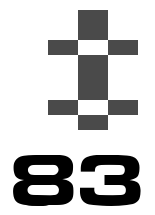
\includegraphics[height=1.0cm]{src/surface_character_mini_diagrams/7_83.png}}
\end{figure}
\vspace{-0.4cm}

\clearpage
\vspace{-0.595cm}
\begin{figure}[H]
    \hspace{0.41cm}
    \begin{adjustbox}{height=1.8cm,right}
      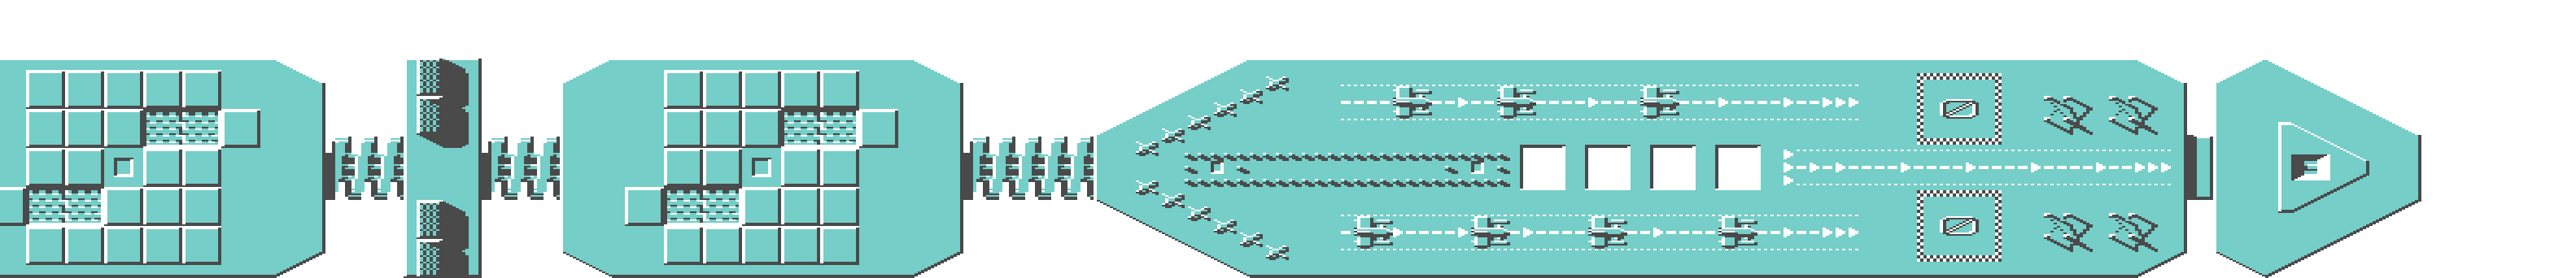
\includegraphics{src/surface_diagrams/7_horizontal_2.png}%
    \end{adjustbox}
\end{figure}
\vspace{-0.4cm}

The bevelled square on the left hand side - 
\raisebox{-0.2\totalheight}{
\includegraphics[height=0.4cm]{src/surface_characters/7_23.png}}
\raisebox{-0.2\totalheight}{
\includegraphics[height=0.4cm]{src/surface_characters/7_26.png}}
\raisebox{-0.2\totalheight}{
\includegraphics[height=0.4cm]{src/surface_characters/7_29.png}}
\raisebox{-0.2\totalheight}{
\includegraphics[height=0.4cm]{src/surface_characters/7_22.png}}
\raisebox{-0.2\totalheight}{
\includegraphics[height=0.4cm]{src/surface_characters/7_25.png}}
\raisebox{-0.2\totalheight}{
\includegraphics[height=0.4cm]{src/surface_characters/7_28.png}}
\raisebox{-0.2\totalheight}{
\includegraphics[height=0.4cm]{src/surface_characters/7_21.png}}
\raisebox{-0.2\totalheight}{
\includegraphics[height=0.4cm]{src/surface_characters/7_24.png}}
\raisebox{-0.2\totalheight}{
\includegraphics[height=0.4cm]{src/surface_characters/7_27.png}}
- likewise uses a combination of tiles similar to the bevel in the previous level - 
\raisebox{-0.2\totalheight}{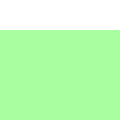
\includegraphics[height=0.4cm]{src/surface_characters/5_26.png}}
\raisebox{-0.2\totalheight}{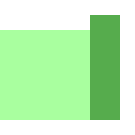
\includegraphics[height=0.4cm]{src/surface_characters/5_29.png}}
\raisebox{-0.2\totalheight}{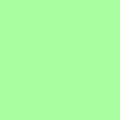
\includegraphics[height=0.4cm]{src/surface_characters/5_25.png}}
\raisebox{-0.2\totalheight}{
\includegraphics[height=0.4cm]{src/surface_characters/5_28.png}}
. The main difference lies only in the color scheme. When we look at the bitpairs forming
the tiles, the principle is the same and essentially the same definition for these
lower numbered tiles, which define common surface elements, is shared between the levels. 

\begin{figure}[H]
    \centering
\raisebox{-0.3\totalheight}{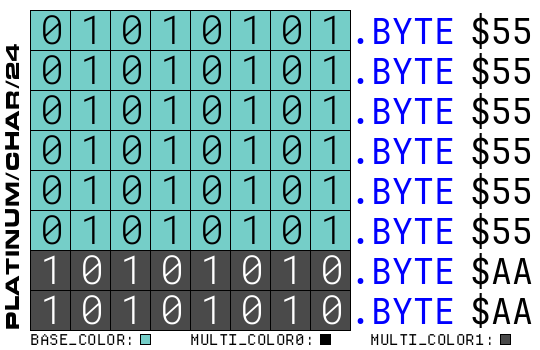
\includegraphics[width=6.3cm]{src/character_set_diagrams/7_24.png}}
\raisebox{-0.3\totalheight}{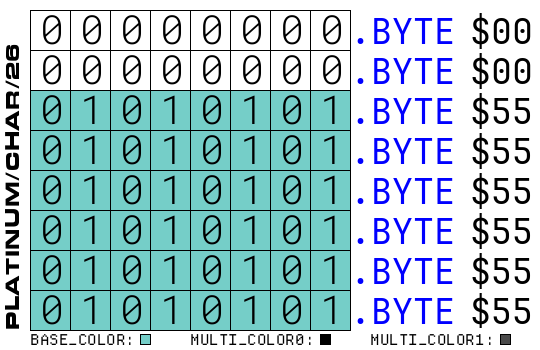
\includegraphics[width=6.3cm]{src/character_set_diagrams/7_26.png}}
\end{figure}
\vspace{-0.4cm}
\begin{figure}[H]
    \centering
\raisebox{-0.3\totalheight}{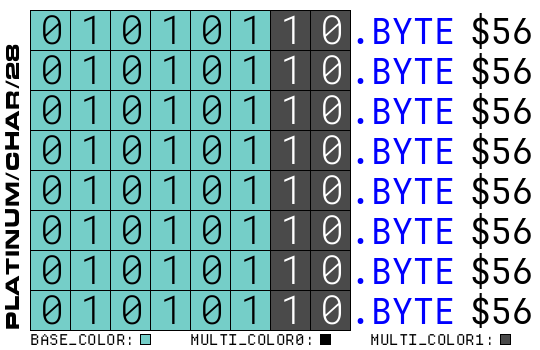
\includegraphics[width=6.3cm]{src/character_set_diagrams/7_28.png}}
\raisebox{-0.3\totalheight}{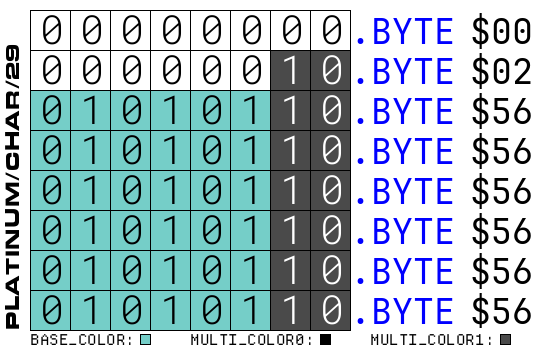
\includegraphics[width=6.3cm]{src/character_set_diagrams/7_29.png}}
\end{figure}
\vspace{-0.4cm}

As we shall shortly see this isn't true for all tiles, particularly those that define structures
placed on the surface.
\clearpage

%\begin{figure}[H]
%    \centering
%    \begin{adjustbox}{width=14cm,center}
%      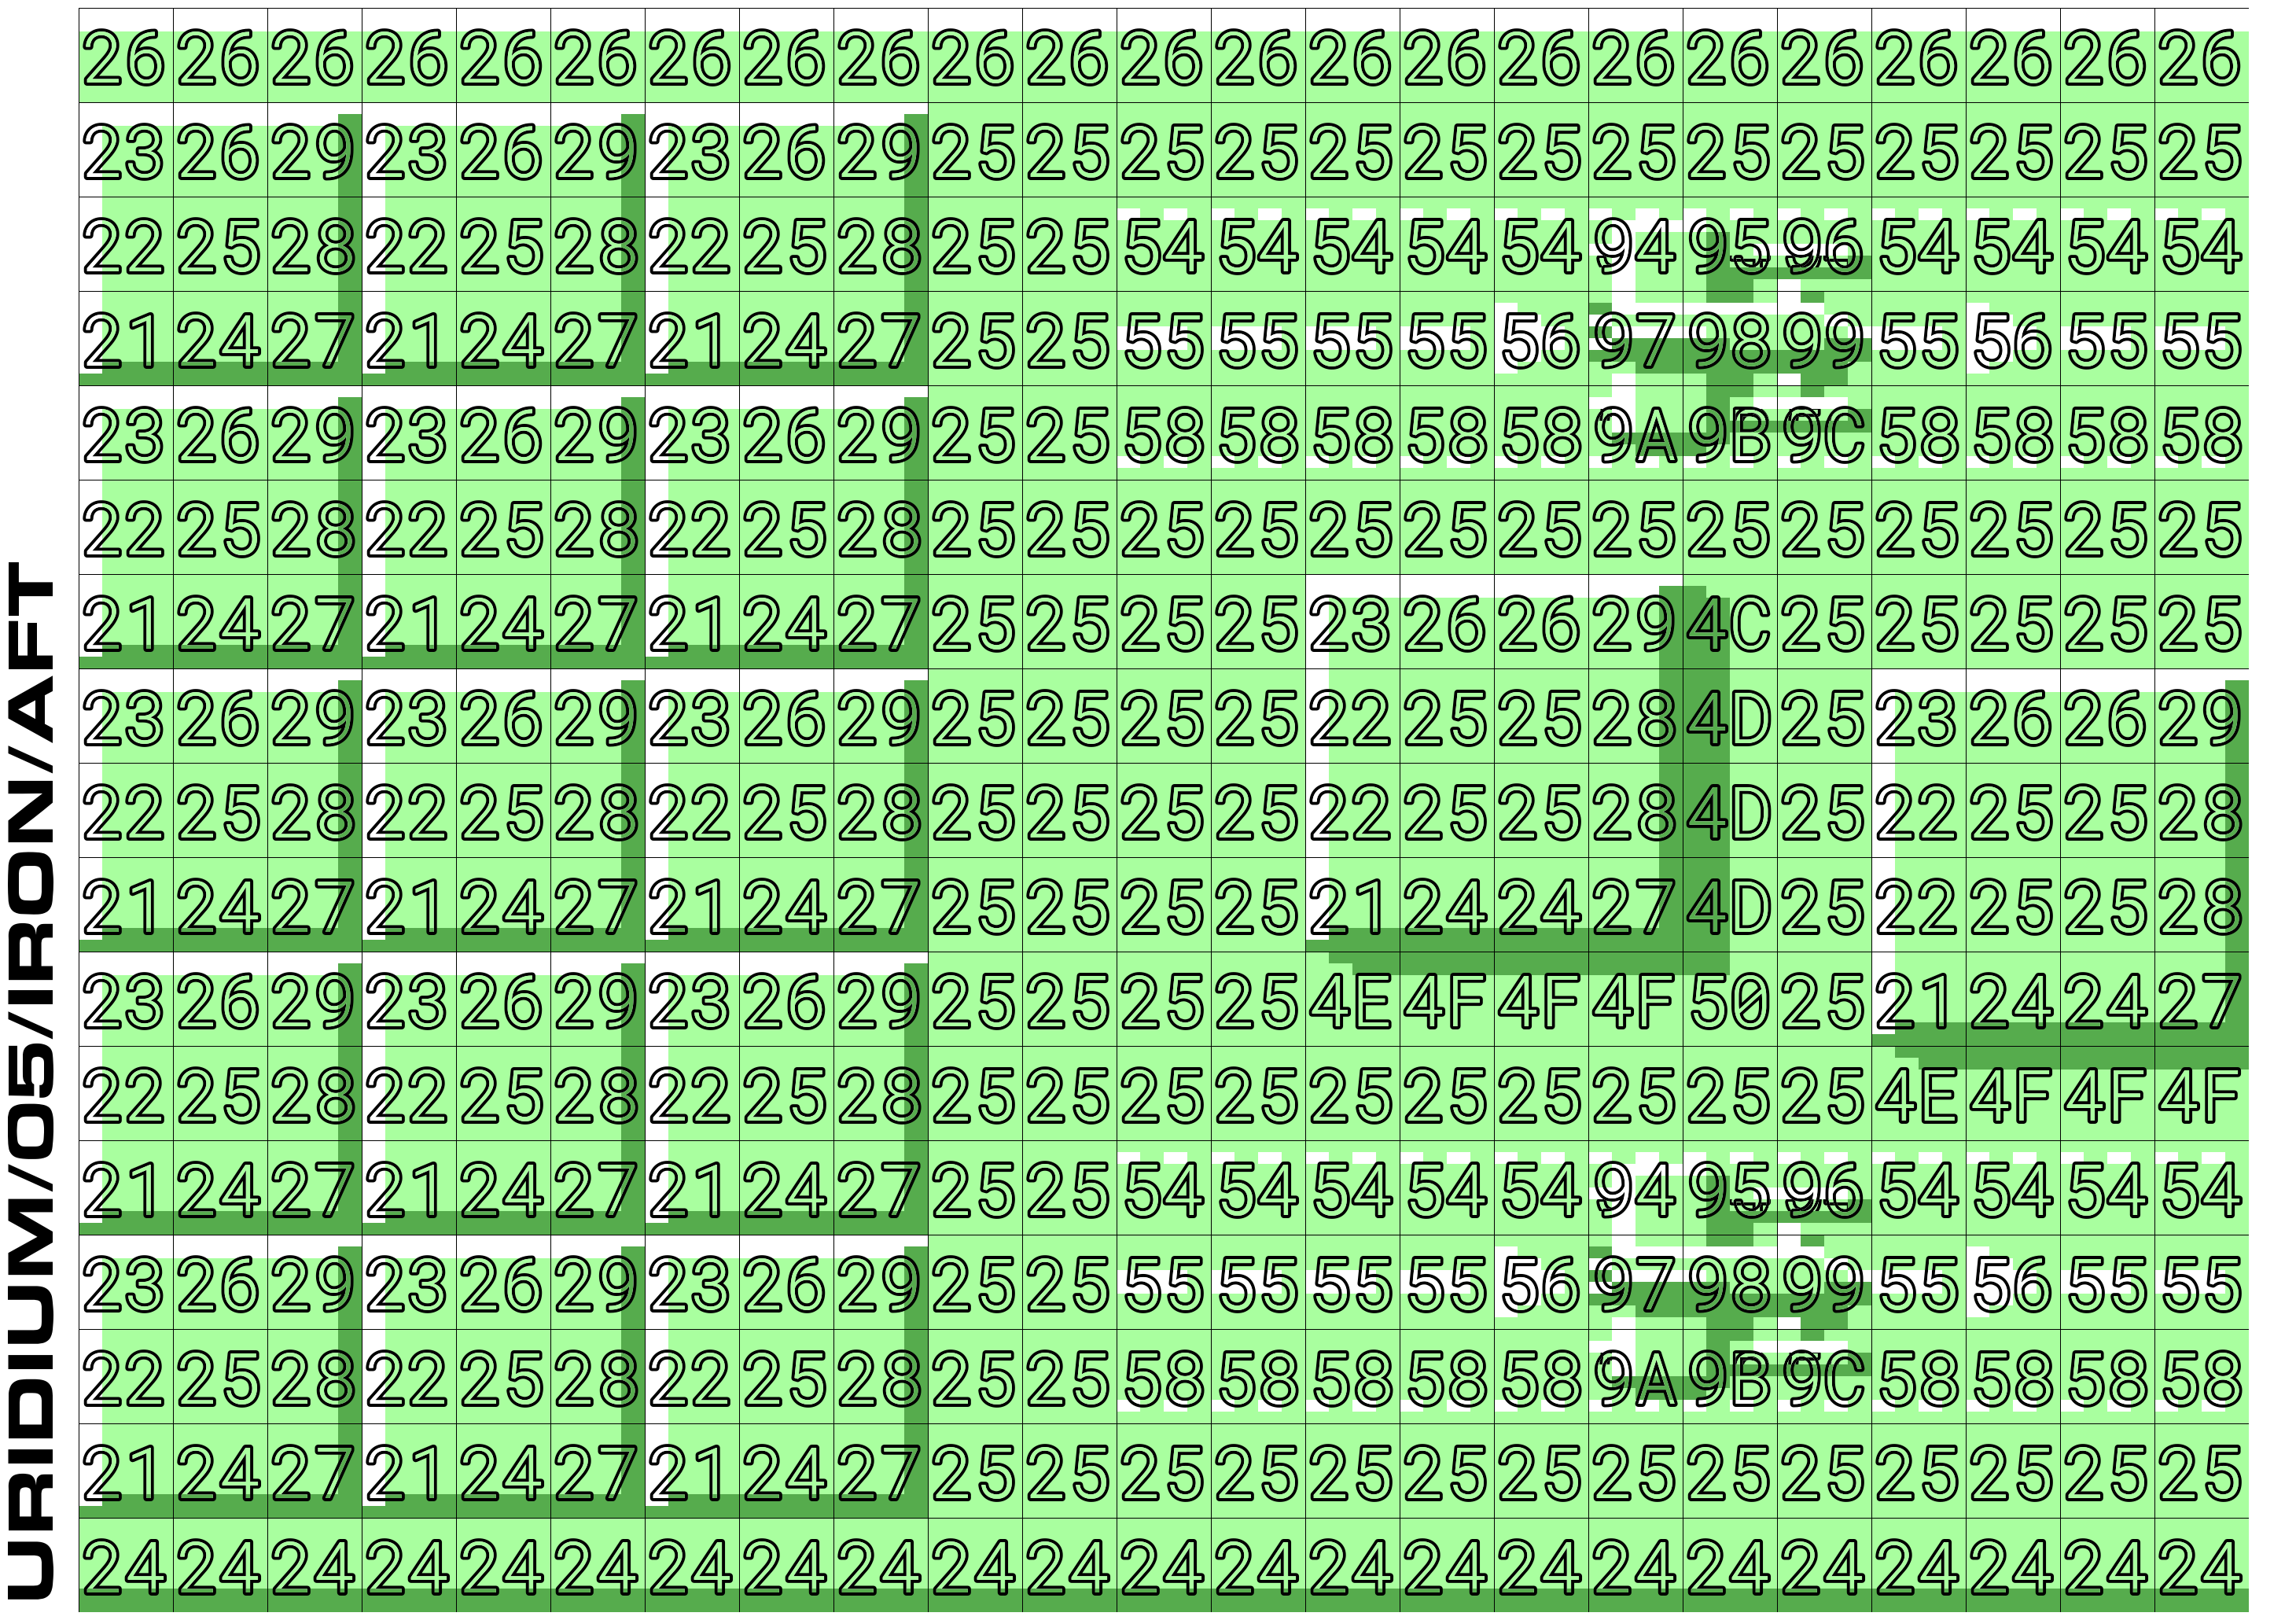
\includegraphics[width=15cm]{src/section_diagrams/5_AFT.png}%
%    \end{adjustbox}
%\end{figure}
%
%\raisebox{-0.3\totalheight}{
\includegraphics[height=1.0cm]{src/surface_character_mini_diagrams/5_5B.png}}
%\hspace{0.1cm}
%\raisebox{-0.3\totalheight}{
\includegraphics[height=1.0cm]{src/surface_character_mini_diagrams/5_5C.png}} %\hspace{0.1cm}
%\raisebox{-0.3\totalheight}{
\includegraphics[height=1.0cm]{src/surface_character_mini_diagrams/5_5D.png}}
%\hspace{0.1cm}
%\raisebox{-0.3\totalheight}{
\includegraphics[height=1.0cm]{src/surface_character_mini_diagrams/5_26.png}}
%\hspace{0.1cm}
%\raisebox{-0.3\totalheight}{
\includegraphics[height=1.0cm]{src/surface_character_mini_diagrams/5_25.png}}
%\hspace{0.1cm}
%\raisebox{-0.3\totalheight}{
\includegraphics[height=1.0cm]{src/surface_character_mini_diagrams/5_2D.png}}
%\hspace{0.1cm}
%\raisebox{-0.3\totalheight}{
\includegraphics[height=1.0cm]{src/surface_character_mini_diagrams/5_2F.png}}
%\hspace{0.1cm}
%\raisebox{-0.3\totalheight}{
\includegraphics[height=1.0cm]{src/surface_character_mini_diagrams/5_2E.png}}
%\hspace{0.1cm}
%\raisebox{-0.3\totalheight}{
\includegraphics[height=1.0cm]{src/surface_character_mini_diagrams/5_55.png}}
%\hspace{0.1cm}
%\raisebox{-0.3\totalheight}{
\includegraphics[height=1.0cm]{src/surface_character_mini_diagrams/5_BF.png}}
%\hspace{0.1cm}
%\raisebox{-0.3\totalheight}{
\includegraphics[height=1.0cm]{src/surface_character_mini_diagrams/5_DD.png}}
%\hspace{0.1cm}
%\raisebox{-0.3\totalheight}{
\includegraphics[height=1.0cm]{src/surface_character_mini_diagrams/5_DE.png}}
%\hspace{0.1cm}
%\raisebox{-0.3\totalheight}{
\includegraphics[height=1.0cm]{src/surface_character_mini_diagrams/5_5B.png}}
%\hspace{0.1cm}

